\chapter{Three-dimensional assessments are necessary to determine the true, spatially-resolved composition of tissues} \label{chap:chap-2}
\begin{refsection}
     
    %%%% remove the following and add your chapter text here
    \section{Introduction}
    Recent developments in spatial profiling technologies have led to the construction of atlases to characterize cellular and tissue compositions, structure, and the “-omic” (genomic, epigenomic, transcriptomic, proteomic, and metabolomic) landscapes of tissues, organs, and whole organisms\cite{Liu2020High,Ozsolak2011RNA,Pidsley2016Critical,Cheng2016Targeting,Braxton20243D,Bell2024PanIN,Vogelstein2013Cancer,Lin2015Highly,Angelo2014Multiplexed}. These techniques have led to important discoveries regarding changes in cellular composition during development, aging and the progression of diseases such as cancer and cardiovascular disease. Due to technical and financial limitations, current spatial omic methods are designed to evaluate mm$^2$-sized two dimensional (2D) regions\cite{Liu2020High,Bell2024PanIN,Goltsev2018Deep,Kuett2021Three,Eng2019Transcriptome,Xia2019Spatial,Bressan2023dawn}. Recently, teams have developed novel techniques, such as open-top light-sheet, micro-CT, serial section based imaging for 3D tissue mapping\cite{Senter2016Role,Liu2023Engineering,Kiemen2022CODA,Gatenbee2023Virtual}. However, attempts to quantify the amount of information gained in the transition from 2D to 3D have been limited. The purpose of this manuscript is to interrogate the added value of quantitative 3D pathology over classical 2D analysis. Here, to evaluate the loss in information when comparing inter- and intra-sample tissue heterogeneity, we analyze >100 pancreas tissue samples in the form of tissue cores, whole slide images (WSIs), and cm$^3$-sized 3D samples
    Consider a histological section of standard, 4 µm thickness, a 1-mm$^2$ core of a tissue microarray (TMA) represents a volume of tissue of just 0.004 mm$^3$, while a common region size for spatial transcriptomics (6.5 x 6.5 mm$^2$) corresponds to a volume of 0.2 mm$^3$. These volumes represent minuscule fractions of the human organs that they are used to represent. More standard techniques, including whole slide images (WSIs) stained with hematoxylin and eosin (H\&E) or immunohistochemistry (IHC), are often considered the gold standard of diagnostic anatomic pathology\cite{Fischer2008Hematoxylin,De2010Immunohistochemistry}. These slides feature a lateral area of 2 x 5 cm$^2$, corresponding to a volume of 5 mm$^3$. The implicit assumption of 2D sampling is that the cells within the sampled region, as well as their morphologies, densities, and cellular and non-cellular neighborhoods, are representative of those of the three-dimensional (3D) organs and diseased tissues from which they are obtained. 
    Accurate clinical diagnosis of a range of diseases using single 2D H\&E sections (selectively from gross inspection of resected tissues) shows that generalization of findings from 2D is possible, although recent works suggest that relevant criteria including cancer grade and cancer precursor type may be easily misdiagnosed in 2D\cite{KiemenPanIN,Triage,Winetraub2021OCT2Hist,Liu2023Engineering,Song2023Weakly}. In research settings, where the goal of tissue atlas efforts is generalizability, we hypothesize that 2D sampling may be insufficient to capture the marked intra-sample heterogeneity in cellular composition and tissue architecture.
    Recent 3D work has demonstrated the utility of tissue clearing and serial sectioning-based approaches to assess microanatomical maps of large (>1 cm$^3$) volumes of tissue at cellular resolution\cite{Fischer2008Hematoxylin,Liu2024Engineering,Susaki2014Whole,Hong2020Three,Koyuncu2023Visual,Crawford2024Combined,Kiemen2023Tissue,Bishop2024end,KiemenHighResolution,Tempest2020Histological,Barmpoutis2021Tertiary,Kiemen2024Magnetic,Liu2021Harnessing,Onozato2012role,Langer2019Modeling}. Here, we use the recently developed 3D imaging workflow CODA to assess the spatial composition of key cells types in thick slabs of both grossly normal human pancreas tissue and human pancreas tissue containing pancreatic ductal adenocarcinoma (PDAC), the deadliest form of pancreatic cancer\cite{Kiemen2022CODA}. CODA was recently advanced to enable user interface-guided workflows in an open source programming language\cite{Matos2025CODAvision}, and has been used to quantitatively interrogate normal human organ development, as well as breast cancer, prostate cancer, pancreatic cancer, diabetic neuropathy, myocarditis, skin regeneration and fetal development in murine and human tissues\cite{Crawford2024Combined,Xue2022Mechanical,Yang2022Engineered,Forjaz2025Integration,OBrien2024Skin,Kiemen2023Intraparenchymal,Groot2021Characterization,Sneider2022Deep,Kiemen20243D,Steele2020Multimodal}. The uniquely heterogeneous spatial microenvironment of PDAC makes it an optimal testbed to evaluate the benefits of 3D microanatomic mapping over standard 2D approaches\cite{Steele2020Multimodal,Wang2020Multiparametric,Raphael2017Integrated}.  
    Our exhaustive analysis demonstrates that standard 2D sampling – using a limited number of TMA cores or WSIs  – is typically insufficient for accurate assessment of tissue composition, tumor content, or the selection of regions of interest for creation of TMA cores and capturing rare events\cite{Kiemen2023Intraparenchymal}. We determine that tens of WSIs and hundreds of TMA cores are necessary to accurately represent the range of tissue compositions present in a cm$^3$-sized human pancreas sample. We find that sections inside a tumor, sometimes just tens of microns apart, can have completely different, uncorrelated cellular and non-cellular structures. Two-dimensional assessments of “representative” slides fail particularly in enumeration of rare events, such as estimation of the density of cancer or cancer precursor cells in samples known to have low neoplastic content\cite{Koyuncu2023Visual,Kiemen2023Intraparenchymal}. This work helps clarify the impact of tissue subsampling in study of the composition of normal and malignant tissues, using analysis of 2D and 3D pancreatic human tissue samples as a testbed. 
    
    \section{Results}
    
    \subsection{Construction of cohorts of 2D and 3D microanatomically labelled pancreatic tissue}
    To interrogate the differences between inter-sample and intra-sampled compositional heterogeneity, pancreatic tissue from 149 individuals was retrospectively collected, consisting of 101 samples containing invasive pancreatic cancer and 48 samples containing grossly normal pancreas (Fig. \ref{chapter2_fig1}A). Three cohorts consist of (1) the “2D-WSI” cohort: 64 individual, pathologist-curated WSIs; the “3D-CODA” cohort: fourteen samples containing serially sectioned 3D blocks (seven of which contain invasive pancreatic cancer); and the “TMA” cohort: a single TMA containing pancreas histology from 30 individuals. Cohorts were matched between the TMA, WSI, and 3D cohorts, according to age and gender (Table S1).

    
    \begin{table}[htbp]
        \centering
        % \footnotesize
        \scriptsize
        \renewcommand{\arraystretch}{1.2}
        \caption{Summary of analyzed pancreatic specimen information. Related to Fig. \ref{chapter2_fig1}}
        \label{table_S1}
        \begin{tabularx}{\textwidth}{l c c c c c c c c c}
            \toprule
            \textbf{} & \textbf{} &\textbf{\#}  & \textbf{Mean images} & \multicolumn{4}{c}{\textbf{Age}} & \multicolumn{2}{c}{\textbf{Gender}} \\
            \cmidrule(lr){5-8} \cmidrule(lr){9-10}
            \textbf{} & \textbf{n} & \textbf{images} & \textbf{per patient} & \textbf{Min} & \textbf{Max} & \textbf{Median} & \textbf{Mean} & \textbf{Female} & \textbf{Male} \\
            \midrule
            WSI cohort   & 64 & 64   & 1   & 48  & 90  & 67    & 64.4   & 22  & 25 \\
            TMA cohort   & 30 & 60   & 2   & 40  & 84  & 60    & 58.4   & 30  & 30 \\
            3D cohort    & 14 & 5503 & 393 & 41  & 75  & 58    & 61.4   & 6   & 8  \\
            \bottomrule
        \end{tabularx}
    \end{table}
    
    We used a segmentation algorithm to label microanatomical components to a resolution of 1 µm (See Materials and Methods). Independent testing showed an overall accuracy of 93.2\% across all samples (Fig. \ref{chapter2_figS1}1). For the 3D-CODA cohort, image registration was performed to create digital tissue volumes (Fig. \ref{chapter2_fig1}B). The minimum number of sections for these 3D samples was 270 (mean: 297, interquartile range: 816). The median reconstructed volume was 39.0 mm$^3$ (mean: 132.2 mm$^3$, interquartile range: 247.3 mm$^3$). Statistical sampling was conducted on the 2D and 3D cohorts to evaluate the impact of sampling on tissue composition analysis of heterogeneous microanatomical tissue components (Fig. \ref{chapter2_fig1}C).

    \begin{figure}[h!]
        \begin{center}
            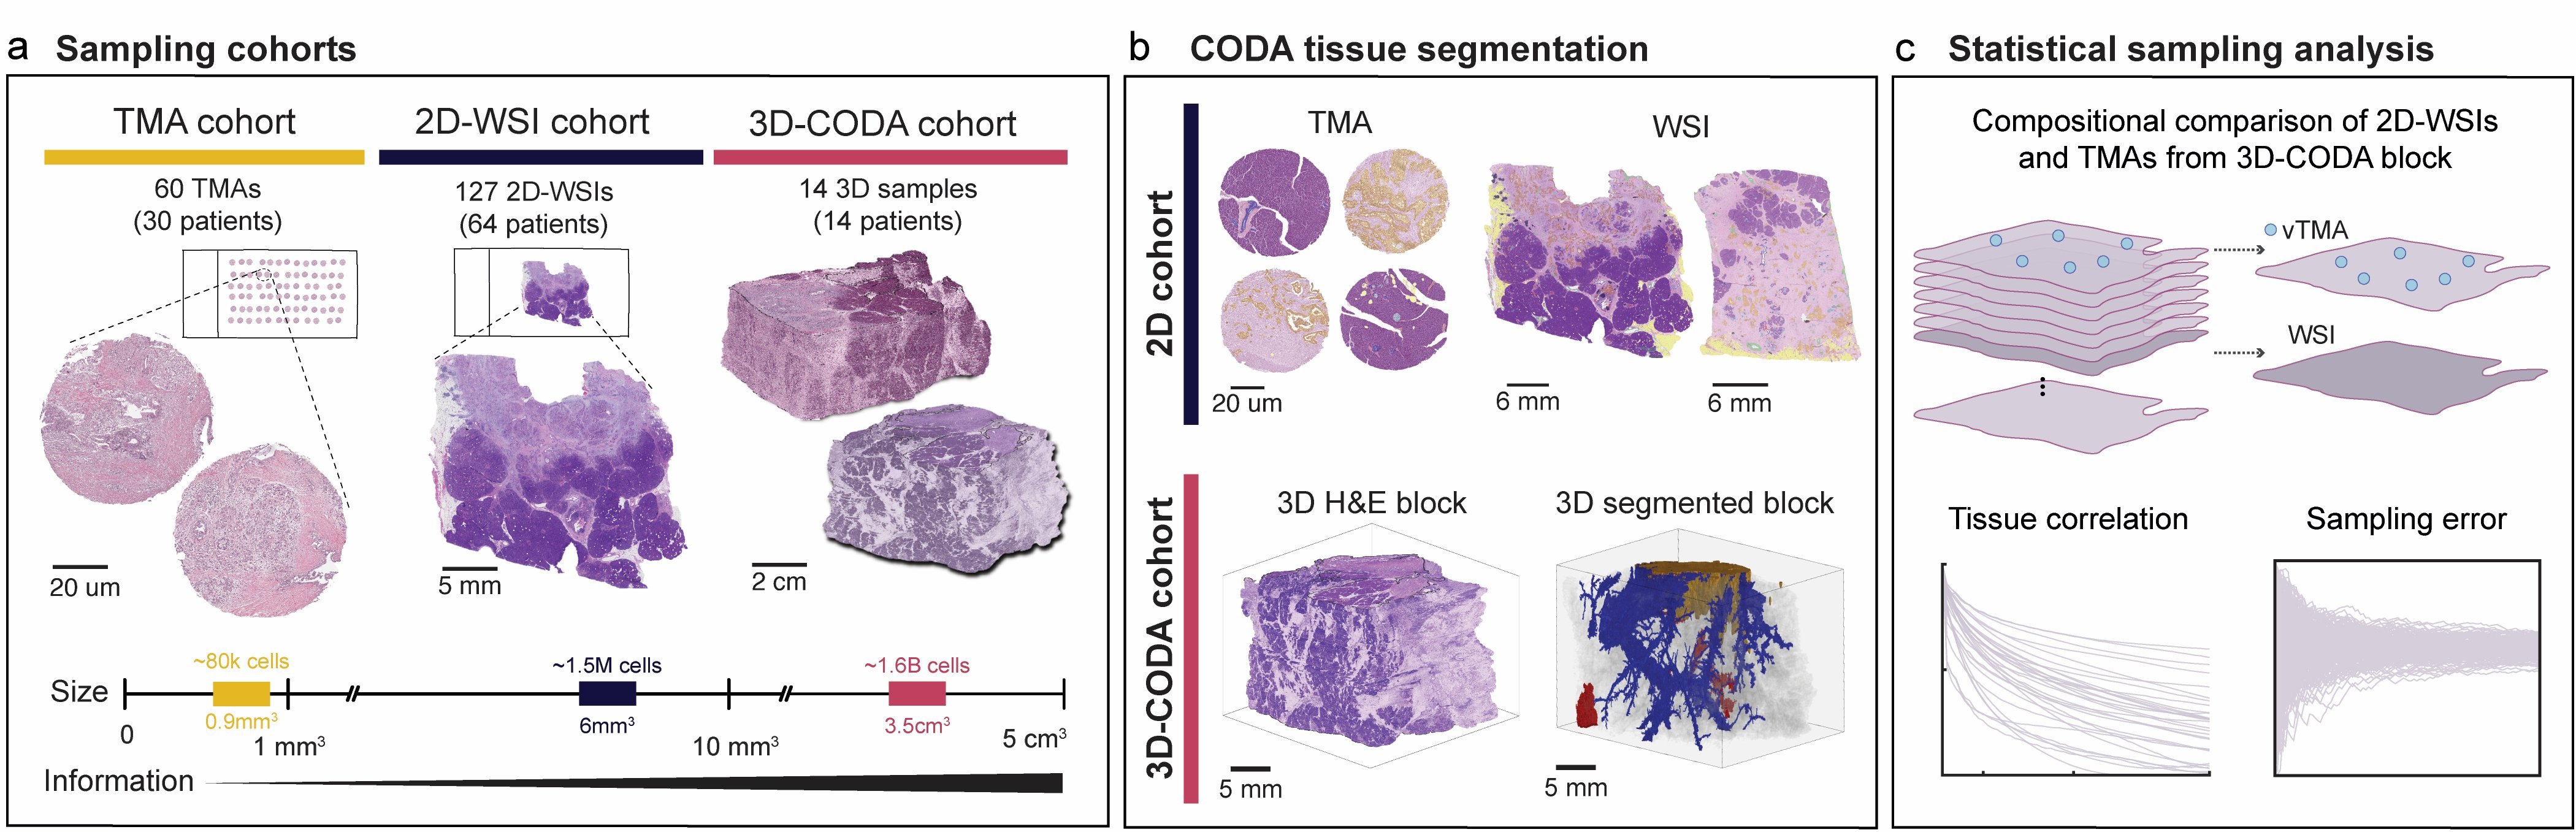
\includegraphics[width=\textwidth,clip,page=1] {figures/chapter2/PDAC_Fig_1.jpg}
            \caption{\textbf{Overview of statistical sampling analysis for assessment of inter- and intra-patient tumor heterogeneity.} (a) Cohorts of 14 3D blocks, 127 WSIs from 64 individuals, and a TMA containing cores from 30 samples were collected. (b) Tissues were surgically resected, formalin-fixed and paraffin embedded, sectioned, stained with H\&E, and digitized. CODA segmentation was used to label 10 different microanatomical components at a resolution of 1 micron. For the processing of the 3D-CODA cohort, specimens were additionally registered into aligned tissue volumes. (c) Statistical sampling analysis was conducted to assess the importance of sampling and associated sampling error.}
            \label{chapter2_fig1}
        \end{center}
    \end{figure}
    
    \begin{figure}[h!]
        \begin{center}
            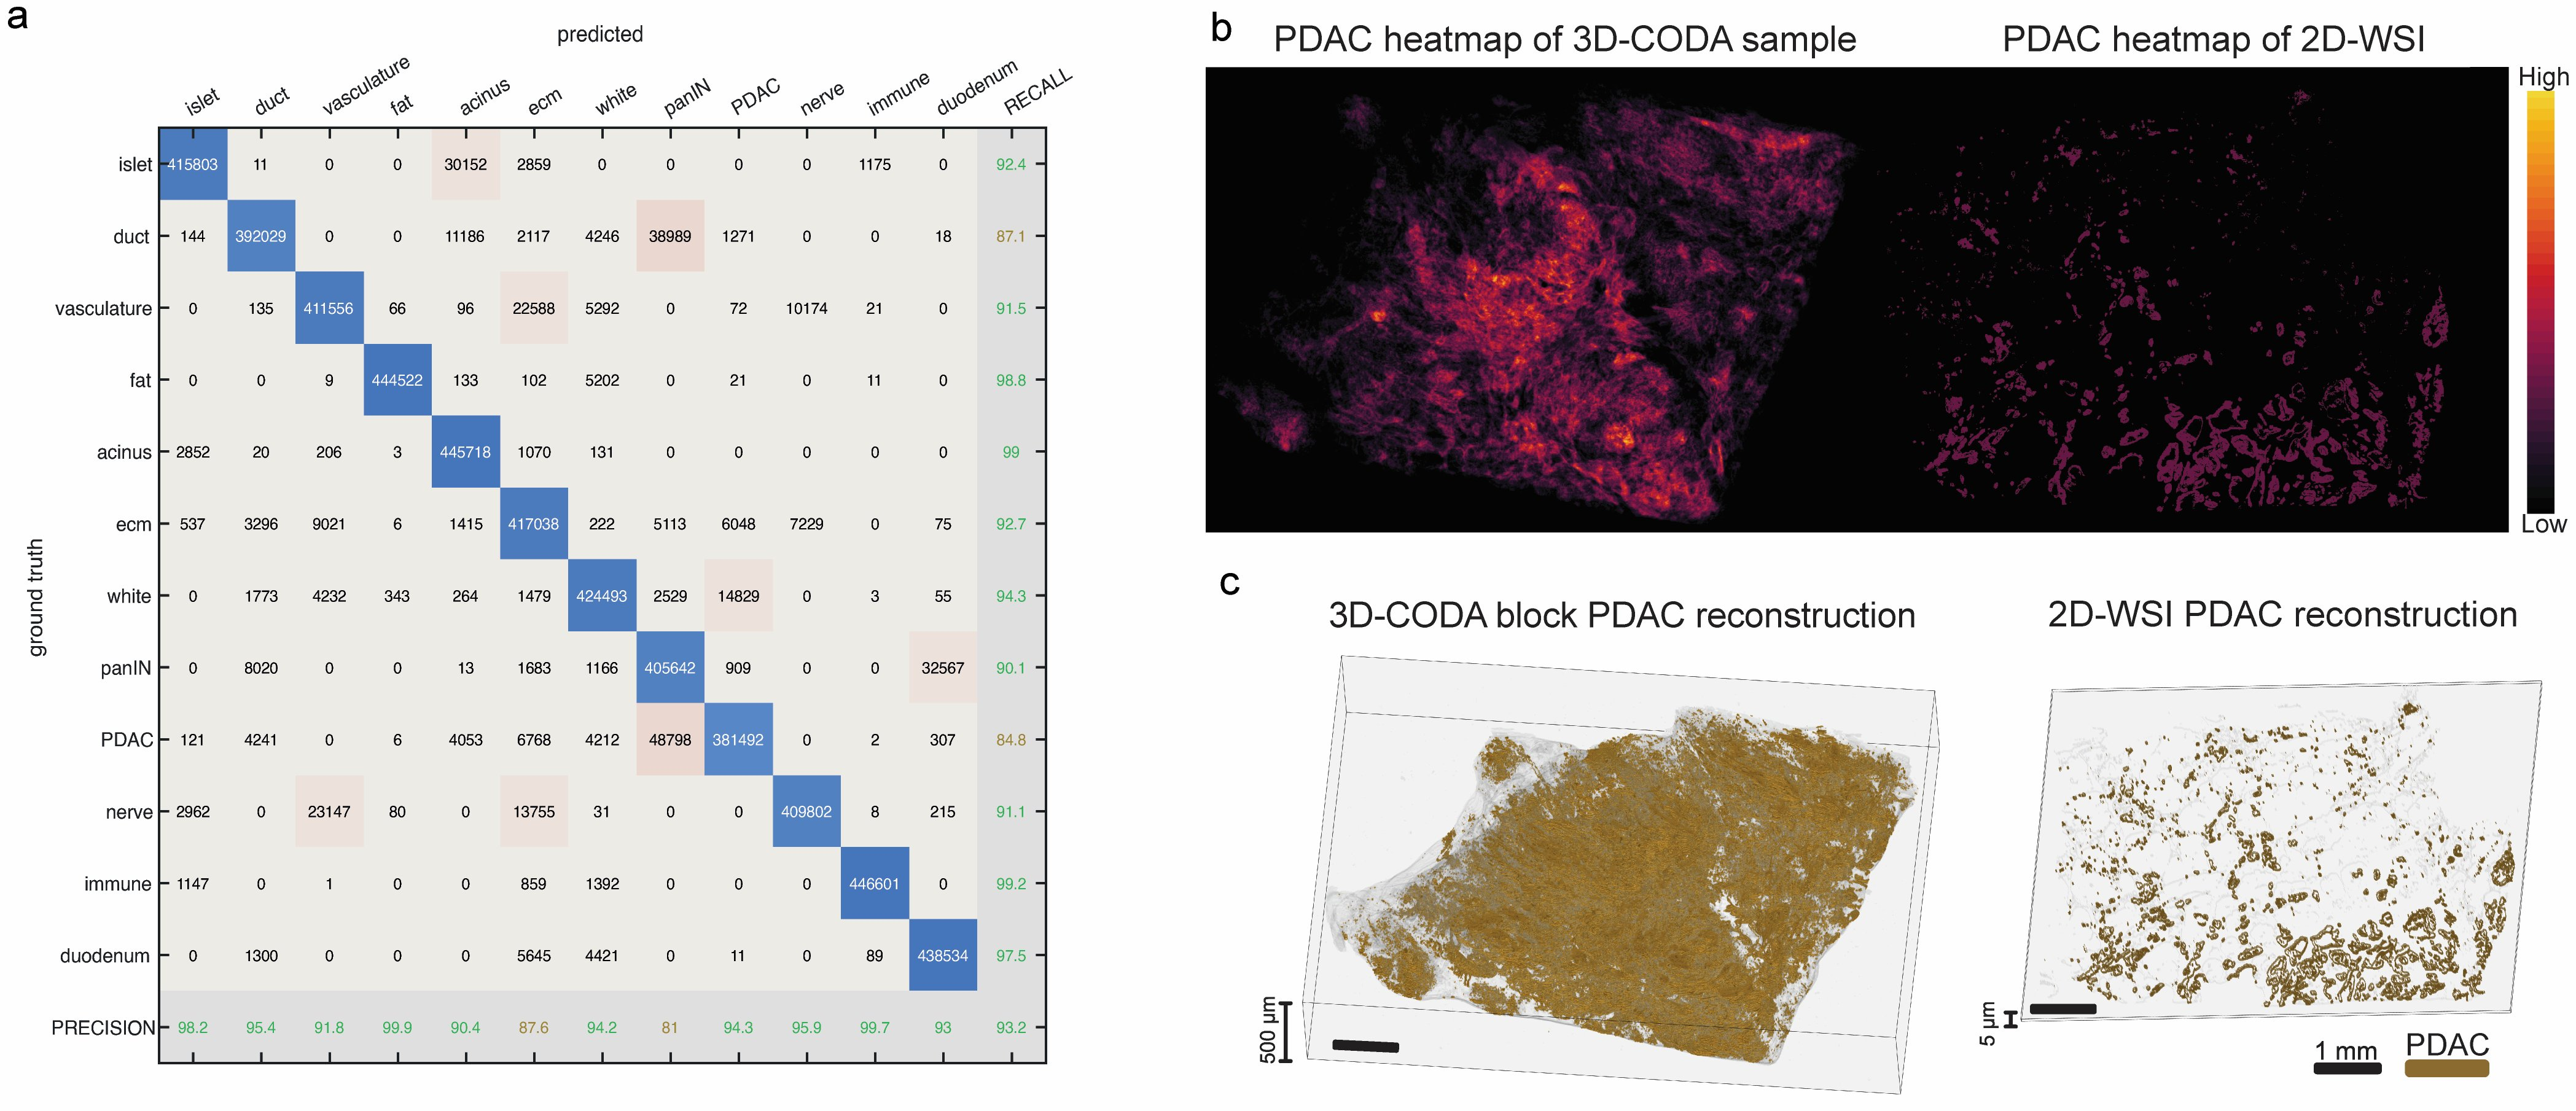
\includegraphics[width=\textwidth,clip,page=1] {figures/chapter2/PDAC_Fig_S1.jpg}
            \caption{\textbf{Validation of deep learning segmentation of pancreatic microarchitecture.} (a) Confusion matrix representing the overall accuracy and per-class precision and recall of the segmentation algorithm used to map the tissue composition in the 2D and 3D samples. Confusion matrix built using independent manual annotations not used in training. (b) Z-projection of PDAC content in 3D volume as opposed to PDAC content in a single WSI. (c) 3D reconstruction of PDAC content in 3D-CODA block in comparison with single 2D-WSI.}
            \label{chapter2_figS1}
        \end{center}
    \end{figure}
    
    \subsection{Spatial correlation rapidly decays within pancreatic tumors}
    To assess the structural continuity of tissues, we calculated how rapidly tissue composition changed along a straight line through the 3D tumors. To determine the correlation length of each tissue component (PDAC, vasculature, fat, ducts, etc.) – i.e. the distance over which the composition remained significantly correlated – we calculated pixel-to-pixel correlation of these tissue components in 3D (Fig. \ref{chapter2_fig2}A). If this correlation is high, then sampling of a tumor can be sparse. As a limit, if this correlation is perfect, then a 2D section is sufficient to capture the composition of the tumor. 
    This correlation was calculated for each tissue component and for all whole-slide images spaced between 4 µm and 720 µm apart, averaged across the seven 3D tumor samples and plotted as a function of distance (Fig. \ref{chapter2_fig2}B). Making intuitive sense, our analysis revealed that more abundant structures such as ECM and acini remained spatially correlated over large distances within the blocks, requiring >180 slides (or 720 µm) until they reached a spatial correlation that had decreased by >50\%. For sparser tissues, such as nerves and vasculature, this correlation dropped by >50\% within just 24 µm, or six 4-mm-thick slices (Fig. \ref{chapter2_fig2}C).  Hence tissue composition becomes rapidly decorrelated within pancreatic tumors.
    To determine whether this rapid decorrelation holds in non-diseased organs, we conducted a similar analysis in seven 3D samples of grossly normal pancreas. Interestingly, the spatial correlation of ECM dropped more rapidly in normal tissue, with loss of >50\% in just 24 µm (compared to 720 µm in cancer tissue). As expected, we found that the spatial correlation in acinar tissue decayed more slowly in normal pancreas, reflecting the marked acinar atrophy and desmoplastic stromal deposition that occurs in pancreatic cancer.
    We repeated this calculation for samples virtually cut to 6.5 x 6.5 mm$^2$, the area used in some spatial transcriptomics analyses (Fig. \ref{chapter2_figS2}). For tissue components including ducts, PDAC, islets of Langerhans, blood vessels, nerves, and fat, a decrease in spatial correlation of fifty percent was observed within just 40 µm, or 10 sections. 
    In conclusion, tissue composition changes rapidly in both normal and diseased tissues, highlighting the necessity of 3D assessments to fully capture their spatial organization.

    \begin{figure}[h!]
        \begin{center}
            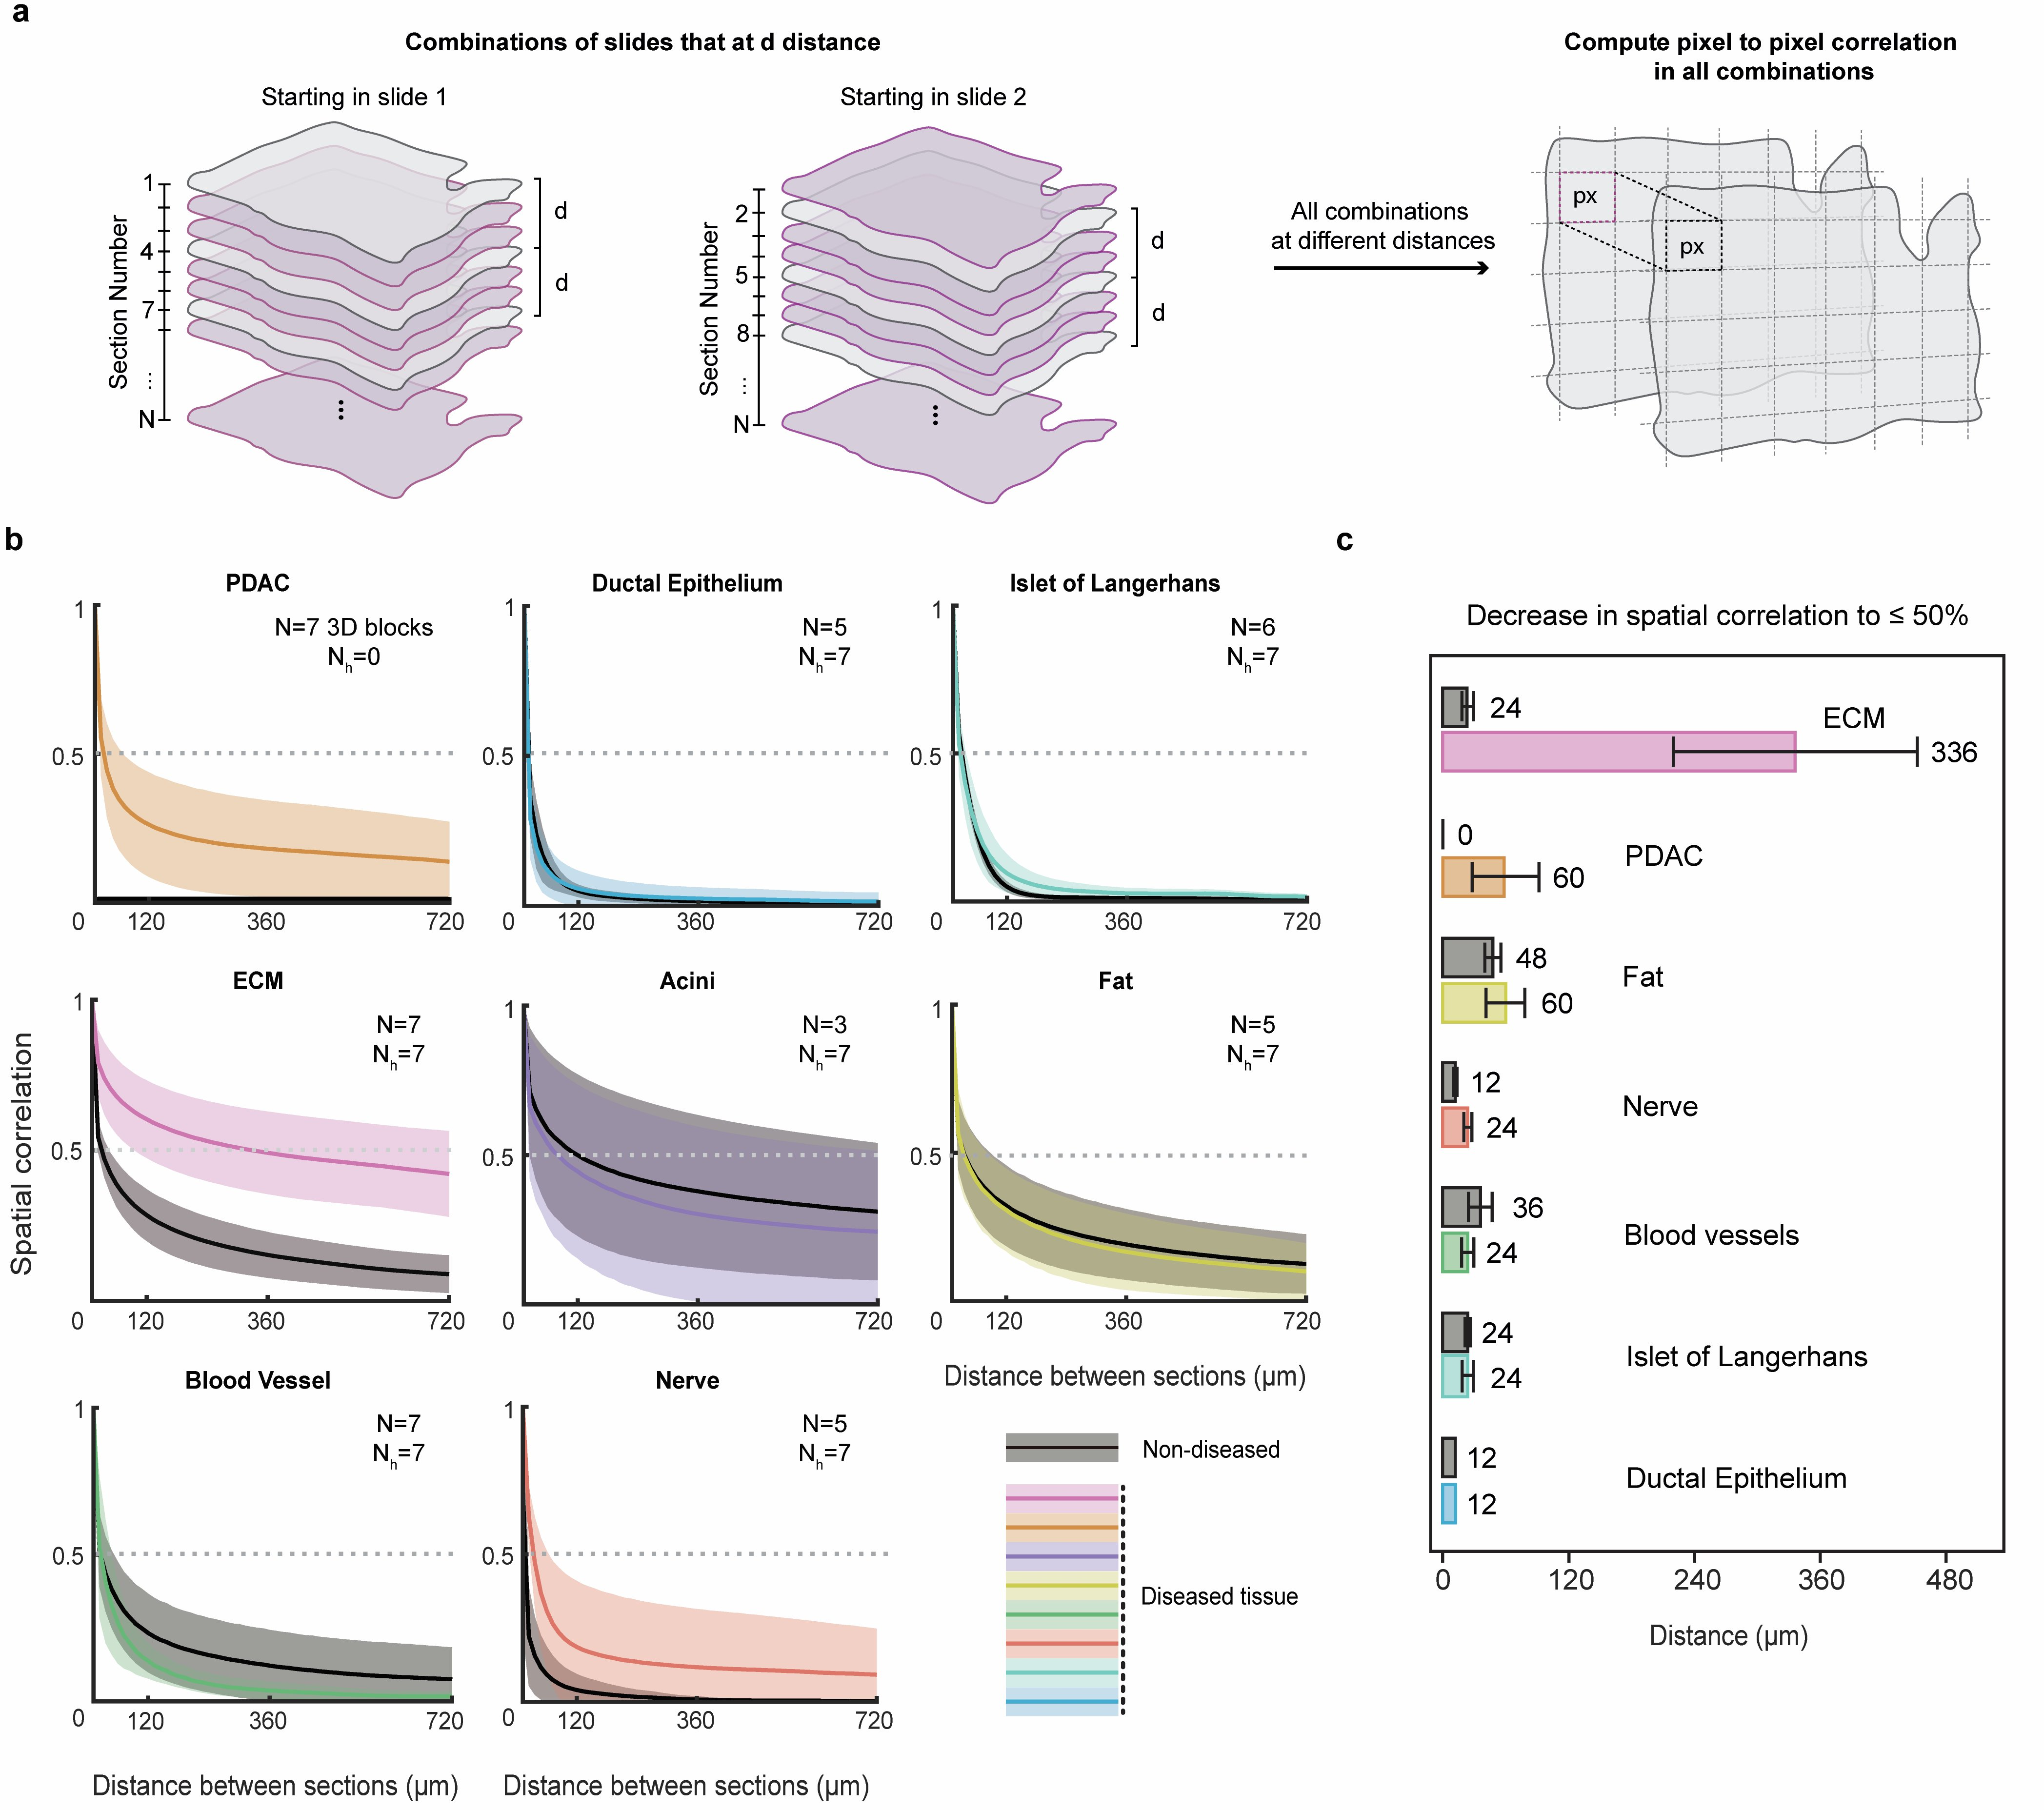
\includegraphics[width=\textwidth,clip,page=1] {figures/chapter2/PDAC_Fig_2.jpg}
            \caption{\textbf{Quantifying the length scale of decay in spatial correlation of tumors.} (a) 2D spatial correlation in tissue composition was determined for all combinations of pairs of sections in the 3D samples. (b) For each tissue type, correlation was plotted as a function of distance between section pairs (line: mean across 3D samples, shaded area: standard deviation across 3D samples; colored plot: cancer samples, grey: grossly normal samples). (c) Distances at which the correlation falls below 50\%, revealing that the length scale of compositional decorrelation in a normal and cancer containing pancreatic tissue is extremely short.}
            \label{chapter2_fig2}
        \end{center}
    \end{figure}
    
    \begin{figure}[h!]
        \begin{center}
            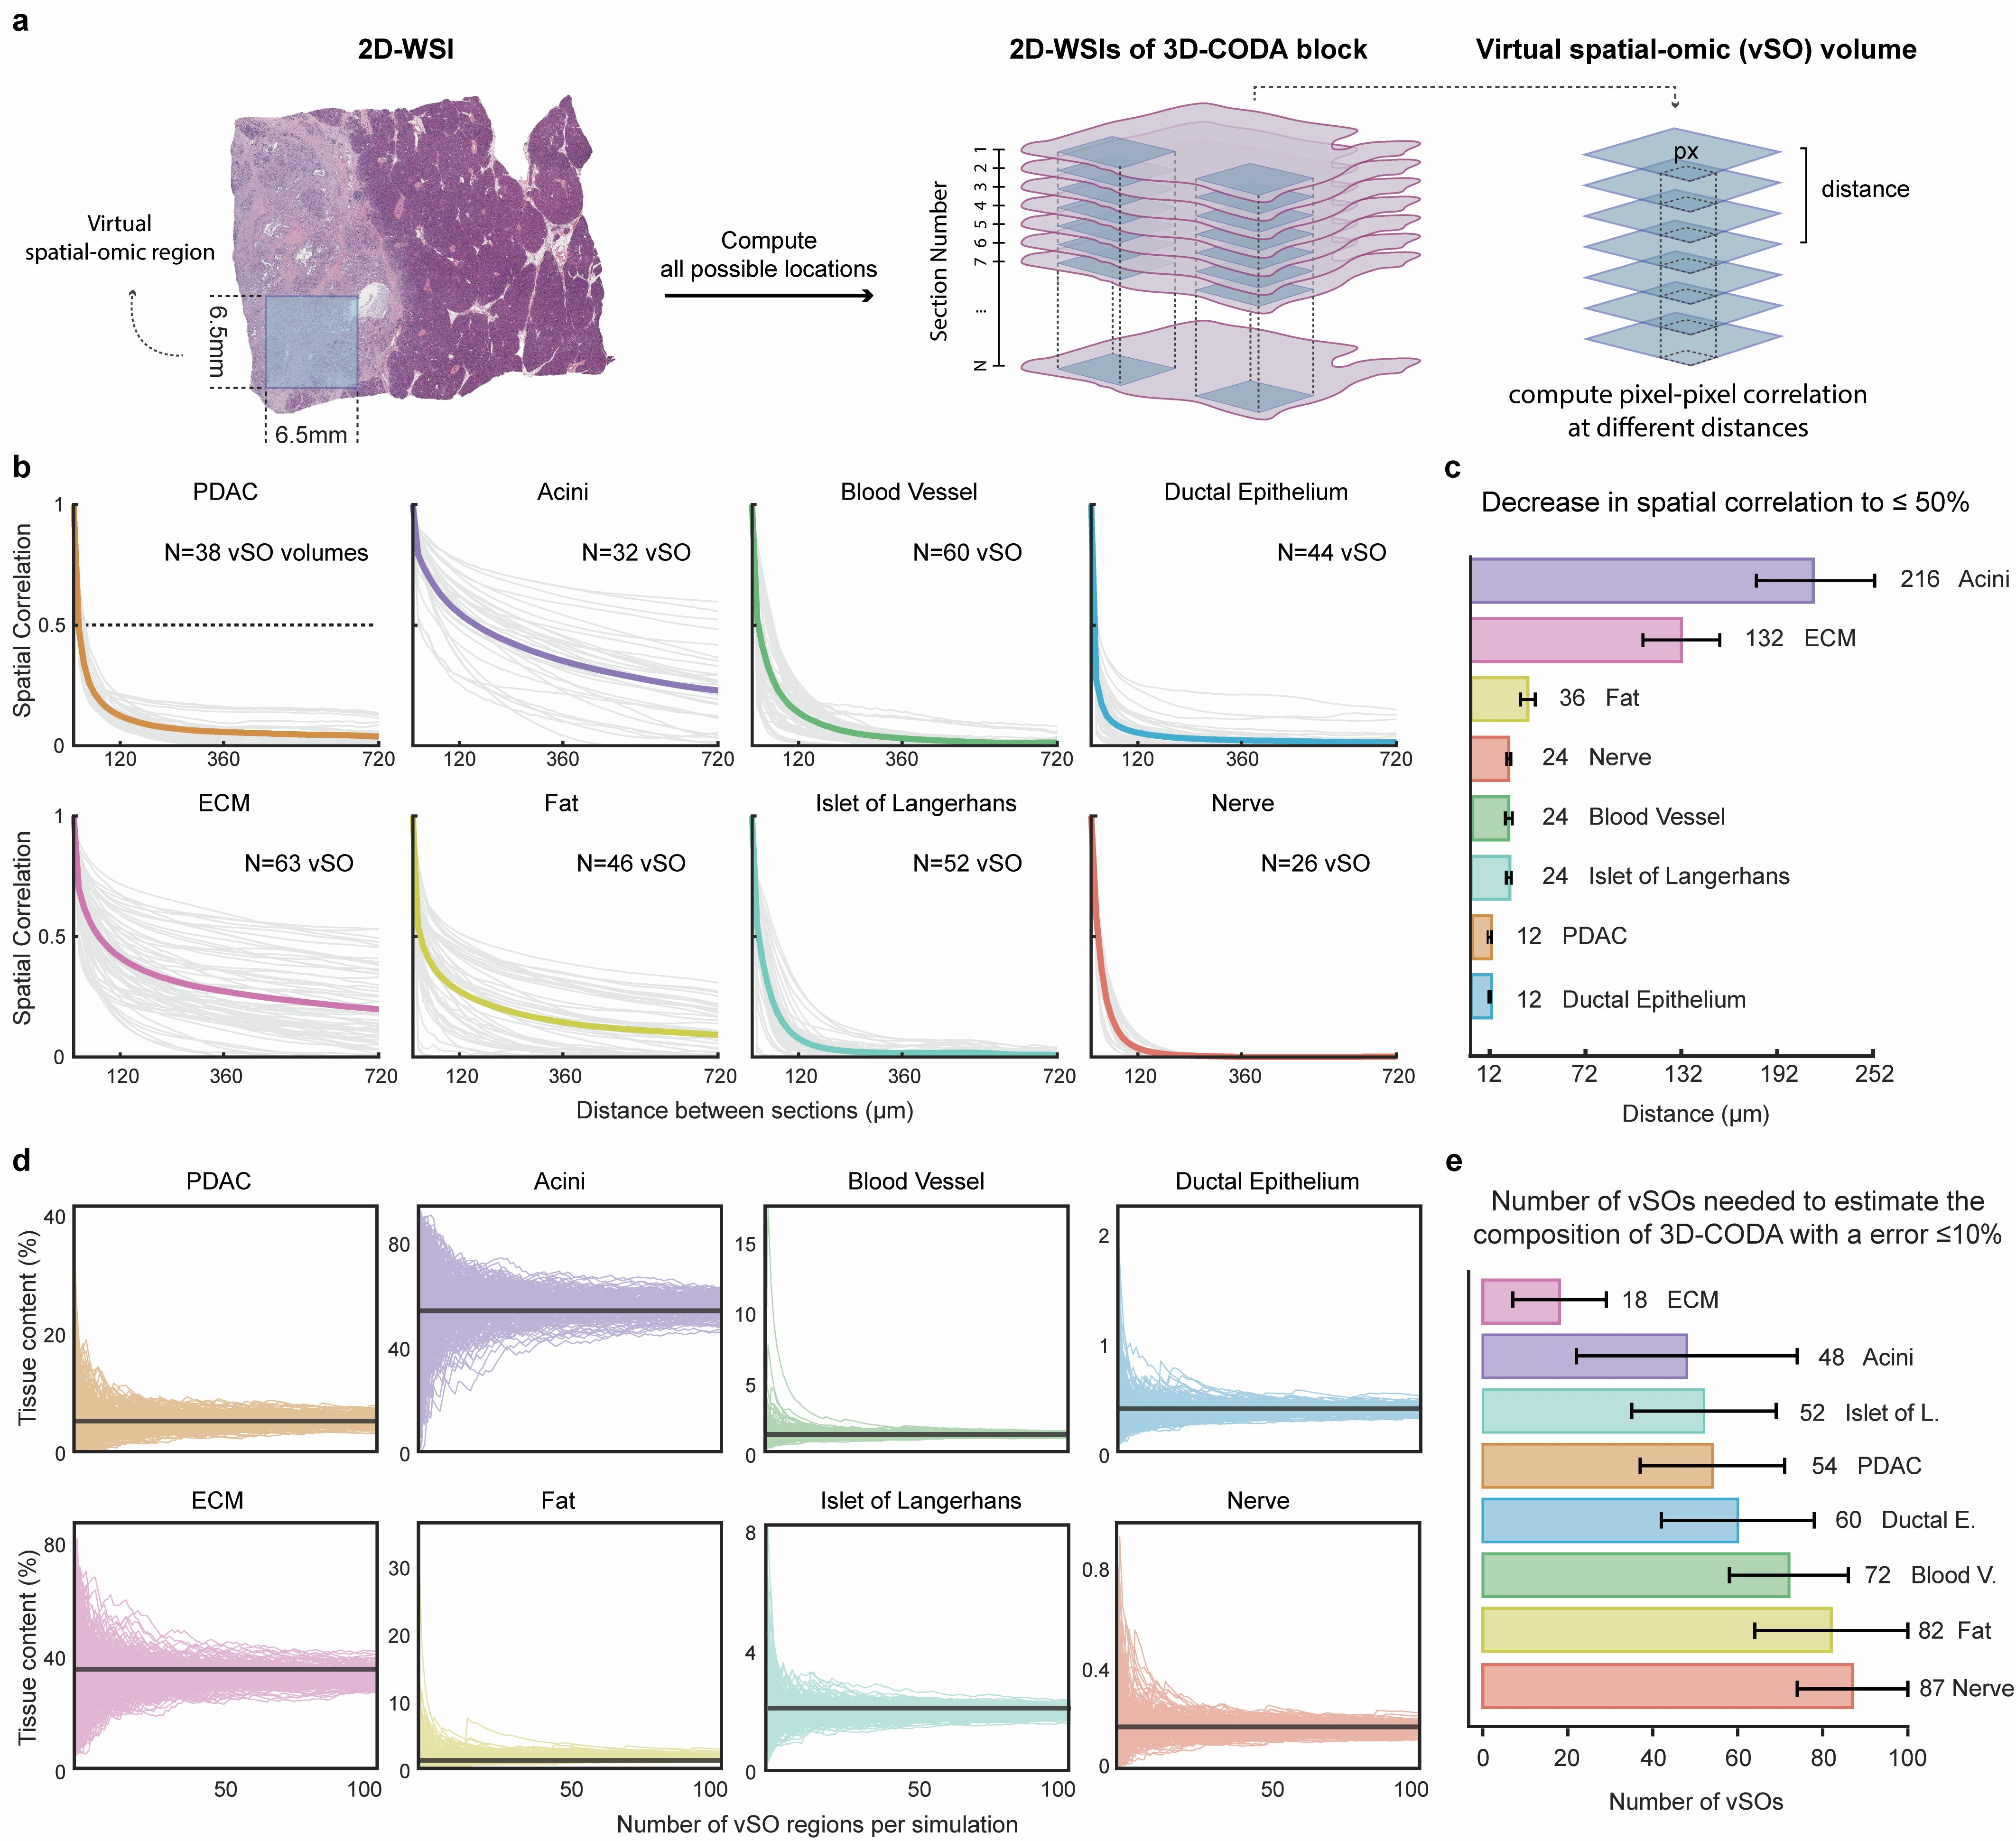
\includegraphics[width=\textwidth,clip,page=1] {figures/chapter2/PDAC_Fig_S2.jpg}
            \caption{\textbf{Quantification of spatial correlation and tissue composition variation at spatial transcriptomics scale.} (a) 65 locations (6.5 x 6.5 mm$^2$) were selected across 7 3D tissue samples. For each, pixel-to-pixel correlation in tissue content was computed for all combination of pairs of spatial-omics size regions. (b) The spatial correlation for each individual region is shown in gray, and the mean of all computations is displayed in color. (c) For tissue components including ducts, PDAC, islets of Langerhans, blood vessels, nerves, and fat, a decrease in spatial correlation of fifty percent was observed within just 40 microns. }
            \label{chapter2_figS2}
        \end{center}
    \end{figure}
    \begin{figure}[h!]
        \ContinuedFloat
        \captionsetup{font=small}
        \caption[]{(d) The loss in the accuracy of tissue composition due to spatial-omic region subsampling was measured through 200 simulations of 1 to 100 virtual spatial-omics (vSOs) in the 3D-CODA cohort. Tissue composition of the generated vSOs was compared to the average 3D-CODA (black line). (e) Between 48 and 72 regions of (6.5 x 6.5 mm$^2$) were required to estimate the tissue composition of components including acini, islets of Langerhans, PDAC, ducts, and blood vessels to within 10\% error.}
    \end{figure}
    
    \subsection{Limitations of core-needle biopsies in assessment of tumor heterogeneity in tissue composition}
    TMAs cores are often created following pathologist-selected regions of interest (ROIs) on a single histological section that contains a target structure (e.g. cancer). Hundreds of sections may be subsequently cut from these cores for use by researchers who aim to study the original structure chosen by the pathologist. We hypothesized that due to the rapid changes in tissue composition across 3D tumors (Fig. \ref{chapter2_fig2}), the specific target structures and cellular features selected by pathologists in the initial ROIs could quickly be lost in the cores as successive sections are cut. To quantify this, we created virtual cores within our 3D samples (Fig. \ref{chapter2_fig3}A). We manually chose 50 locations on the first H\&E section of two 3D samples containing visually high cancer content. From these virtual cores, we digitally cut virtual TMA sections (vTMAs) and quantified the change in tissue composition compared to the first (target) section (Fig. \ref{chapter2_fig3}B). 
    First, we considered the situation where researchers’ objective is to profile the composition of the tumor microenvironment (Fig. \ref{chapter2_fig3}C). We quantified changes in stromal cell density across vTMA sections to assess whether the number and identity of stromal cells would vary greatly between slides, leading to the possibility that two researchers, studying sections from the same TMA cut hundreds of slides apart, could reach opposite conclusions. We found that, as subsequential sections are cut from the initial pathologist-selected ROI, stromal cell density errored on average 25\% within the first 100 sections (0.4 mm), with many simulations nearing 100\% change within 300 sections (~1.2 mm). 
    Finally, we determined the average number of virtual sections within which virtual cores lost their target structure altogether (Fig. \ref{chapter2_fig3}D). In this case, core ROIs were chosen as containing high cancer content. We thus determined, how many of the 100 simulated cores no longer contained cancer for each virtual section. We found that nearly 50\% of cores contained no cancer within 200 sections (0.8 mm), with this number approaching 75\% after 300 sections. 
    This analysis demonstrates a rapid decorrelation in cancer content even within expert-guided cores, suggesting that TMA cores may rapidly lose the benefit of expert-guided ROI selection as sections are cut. 
    
    \begin{figure}[h!]
        \begin{center}
            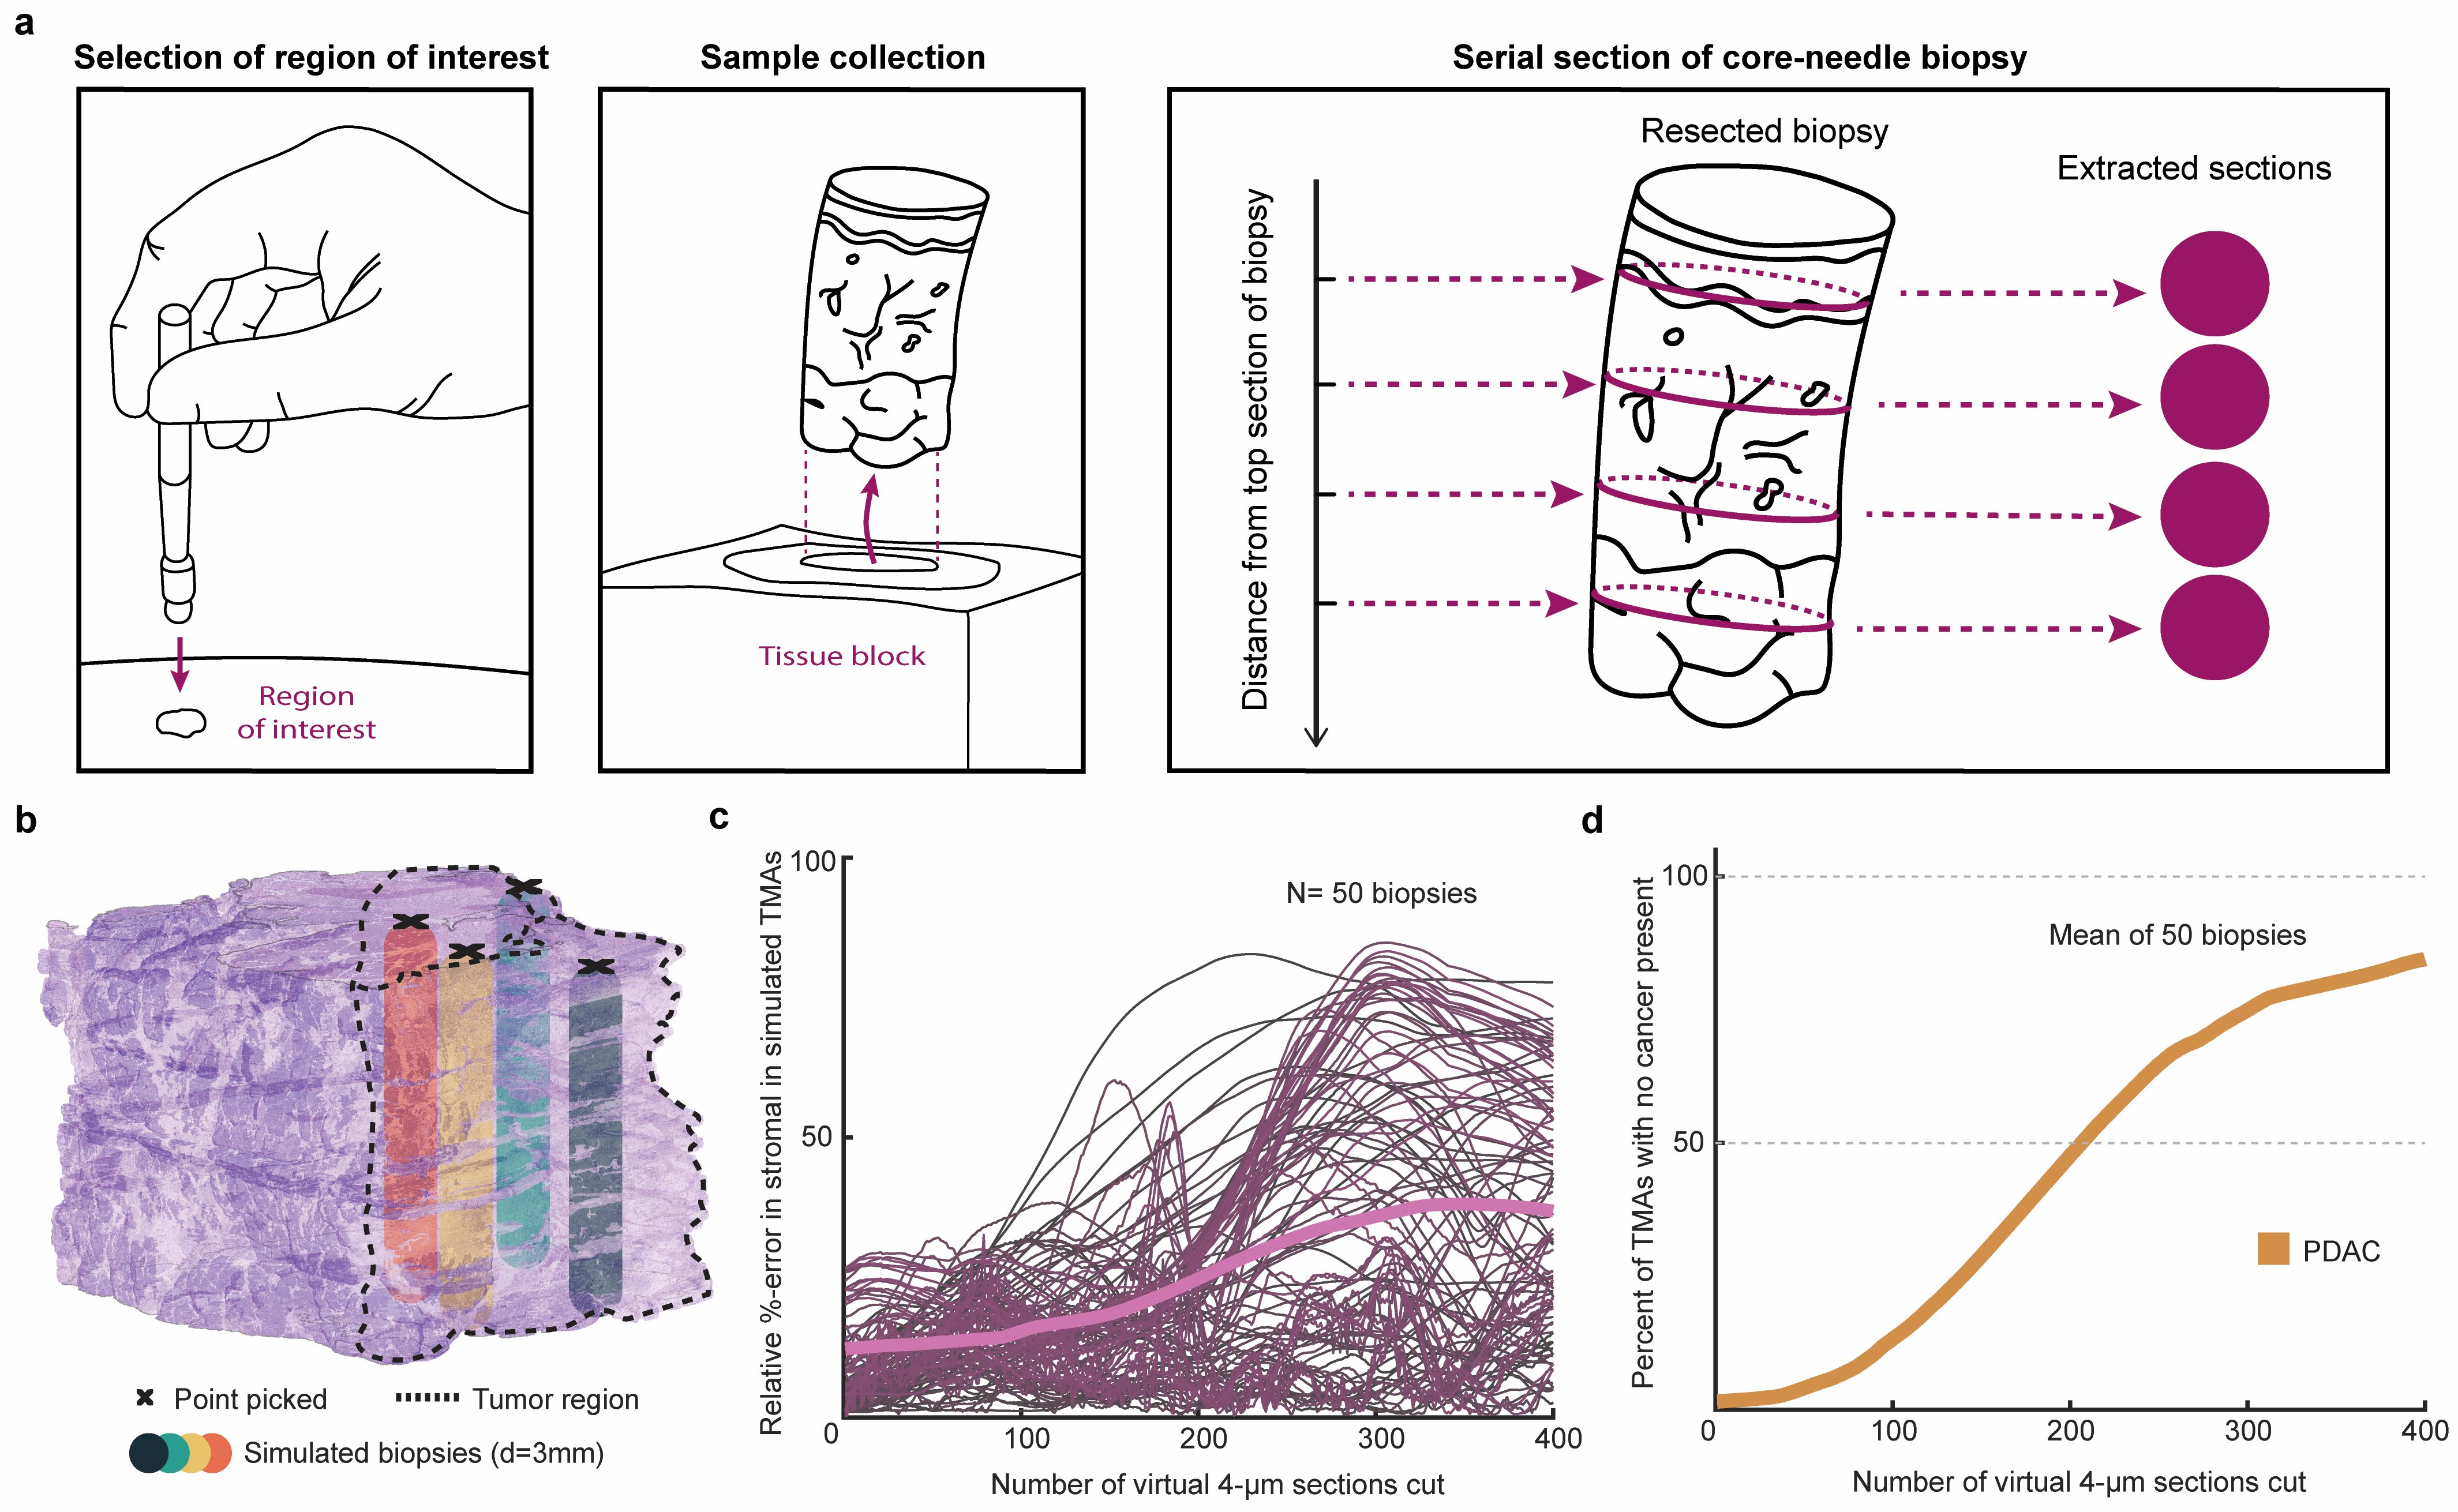
\includegraphics[width=\textwidth,clip,page=1] {figures/chapter2/PDAC_Fig_3.jpg}
            \caption{\textbf{Error when TMA cores are used to assess spatial tissue content in a tumor.} (a) Cartoon demonstrating the process of region selection and tissue coring for creation of TMAs. (b) 50 ROIs containing cancer were manually selected from the top slide of two 3D samples. (c) TMAs were virtually cut and the relative error in stromal cell density in comparison to the original ROI was calculated. (d) TMAs were virtually cut and the percent of TMAs with no cancer present on a given cut was calculated.}
            \label{chapter2_fig3}
        \end{center}
    \end{figure}
    
    \subsection{Hundreds of TMAs are necessary to capture the true tissue composition of WSIs and 3D tumors}
    Conventional histological analysis often relies on 2D tissue sections or TMAs to quantify the overall composition of tumors. While practical for large-scale studies, this approach assumes that these limited samples are representative of entire heterogeneous 3D tumors. This can lead to significant loss of information, which can overlook important spatial tissue composition variations and miss rare cell populations. Here, we aimed to quantify information loss when subsampling a heterogeneous 3D sample through 2D histology. To do this, we randomly simulated virtual TMA (vTMAs) with 1 mm diameter in the 2D WSIs and the 3D samples (Fig. \ref{chapter2_fig4}A). We quantified the error in tissue composition for various numbers of random, non-overlapping vTMAs compared to the true, 3D tissue composition (Fig. \ref{chapter2_fig4}B). This process was repeated to quantify the error between vTMAs and 2D WSI composition (Fig. \ref{chapter2_fig4}C), and the error between 2D WSIs and 3D tissues (Fig. \ref{chapter2_fig4}D). 
    As expected, increasing the number of TMAs taken from a sample decreased the error of estimation of tissue composition of that sample, and this error varied across different microanatomical tissues (Fig . \ref{chapter2_fig4}B-D). By comparing the number of 2D sections necessary to reach <10\% error, we identified tissue components of high and low heterogeneity (Fig . \ref{chapter2_fig4}E-G). We identified ECM as the component with the lowest heterogeneity, with an average of 19 TMAs necessary to reach <10\% error in the estimation of 2D-WSI composition, 22 TMAs necessary for estimation of 3D-volume composition, and only 1 WSI necessary to correctly estimate 3D-volume composition (within 10\% error). In contrast, we identified cancer as a much more heterogeneous structure, with >500 TMAs necessary to estimate the true 3D composition with <10\% error.
    We repeated this calculation for samples virtually cut to 6.5 x 6.5 mm$^2$, the area often used in spatial transcriptomics analyses (Fig. \ref{chapter2_figS2})\cite{Moncada2020Integrating,Johnson2023Digitize,He2020Integrating,Longo2021Integrating}. Our analysis demonstrated that tissue components including acini, islets of Langerhans, PDAC, ducts, blood vessels required roughly 50 simulated sections to estimate true 3D tissue composition with < 10\% error. Overall, this analysis demonstrates that subsampling heterogeneous tumors leads to significant information loss, and that this information loss may be quantified through simulation of 3D anatomical tissue maps.


    \begin{figure}[p]
        \begin{center}
            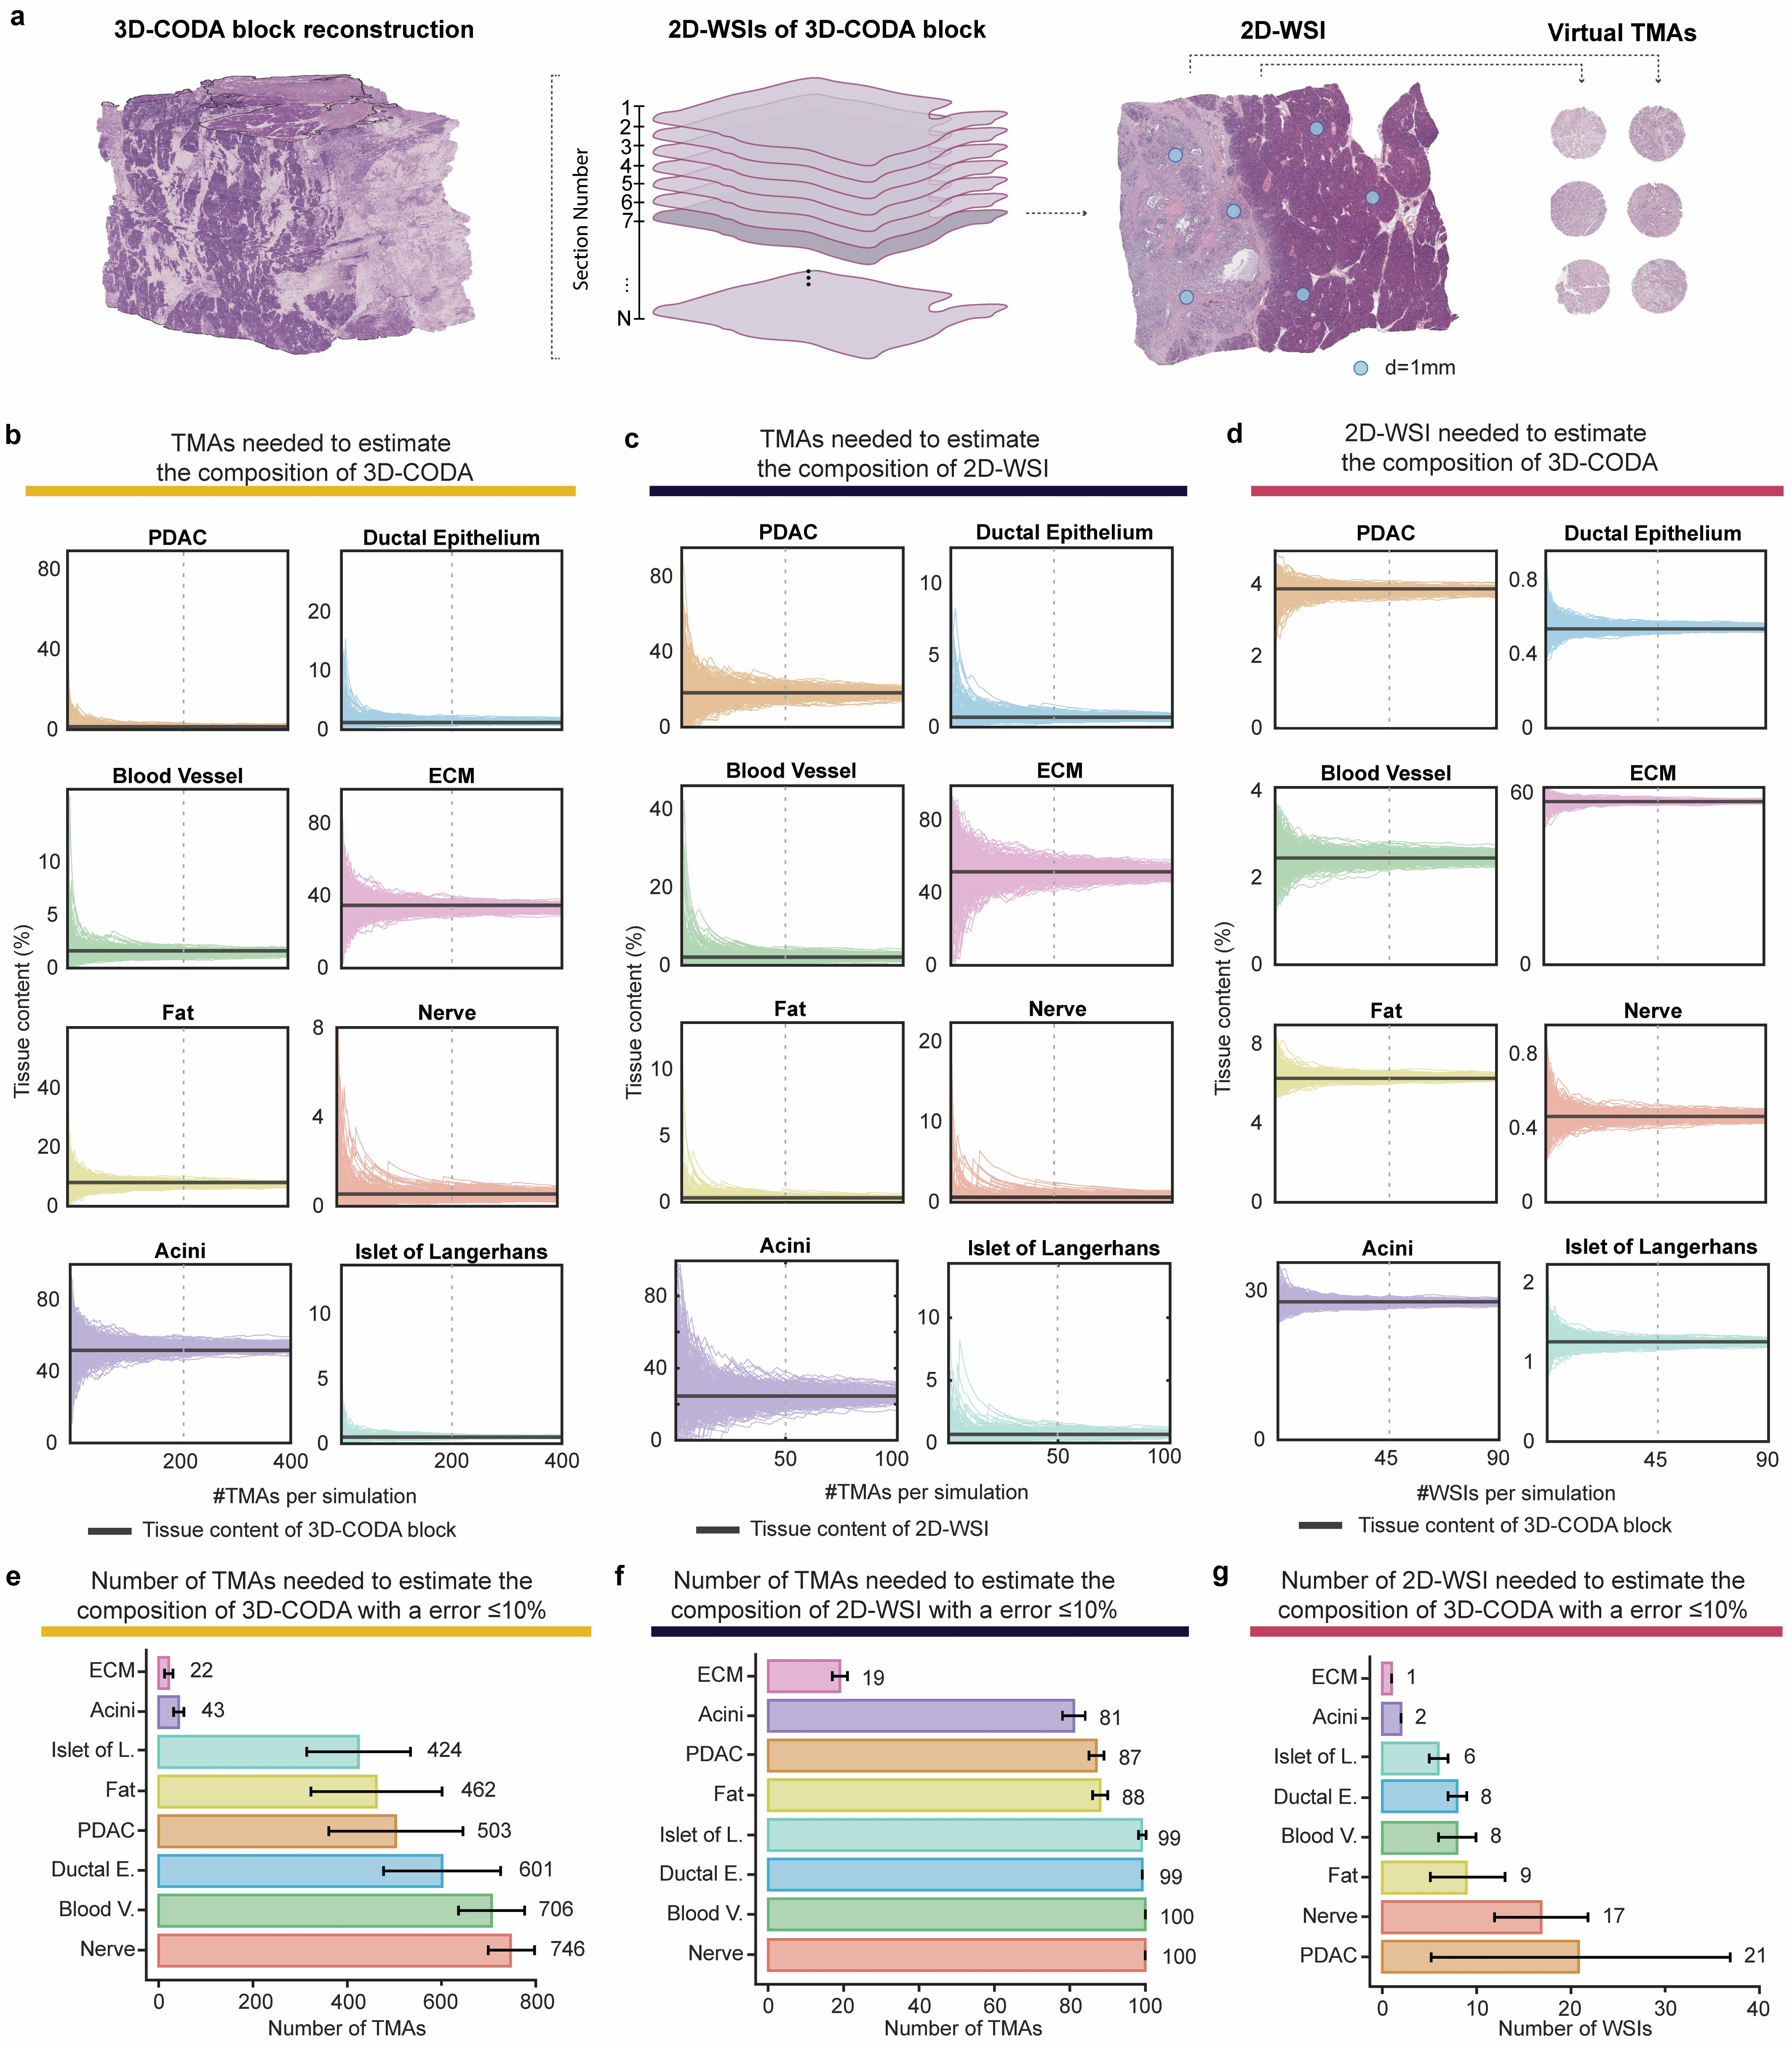
\includegraphics[width=1\textwidth,height=0.9\textheight,keepaspectratio,clip,page=1]{figures/chapter2/PDAC_Fig_4.jpg}
            \captionsetup{font=small}
            \caption{\textbf{Hundreds of TMAs and tens of WSIs are needed to accurately estimate the true composition of 3D tumors.} (a) Representation of 3D-CODA H\&E-stained volume, comprised of serial, 2D-WSIs, from which virtual TMAs may be extracted. (b) The loss in the accuracy of calculation of tissue composition due to TMA subsampling was measured through 200 simulations of 1 to 100 virtual TMAs (vTMAs) in the 2D-WSI cohort.}
            \label{chapter2_fig4}
        \end{center}
    \end{figure}
    
    \begin{figure}[h!]
        \ContinuedFloat
        \captionsetup{font=small}
        \caption[]{Tissue composition of the generated vTMAs was compared to the average 2D-WSI (black line). The calculation of (a) was repeated for calculation of (c) the loss in accuracy between TMAs and 3D tumors, and (d) the loss in accuracy between 2D WSIs and 3D tumors. (e, f, g) Distilling the information from the simulations shown in (a-c), we determined the number of TMAs and WSIs necessary to estimate WSI and 3D-tumor composition with ≤10\% error. Some structures, such as blood vessels, nerves, and PanIN tens to hundreds of 2D sections to reach ≤10\% error.}
    \end{figure}

    \subsection{Sampling guidelines in pancreatic cancer determined through 3D assessment of neoplastic content}
    In studies of pancreatic cancer initiation and its precursors (PanINs), accurate understanding of the number and composition of cancer precursors in the ductal system is necessary to determine the risk of a given precursor lesion to progress to cancer\cite{Distler2014Precursor,Lennon2014Early,McGuigan2018Pancreatic}. Yet, it is not currently feasible to profile entire human pancreases at cellular resolution to quantify all precursors. Here, we demonstrate that the amount of tissue necessary for incidence profiling may be estimated using simulations of 3D tissue. To do this, we assessed the sampling necessary to reach a preset error in the estimation of neoplastic content. 
    For this calculation, we utilized a previously reported cohort of 48 large 3D reconstructed samples of human pancreas tissue containing pancreatic intraepithelial neoplasia (PanIN), the precursors to pancreatic cancer\cite{Braxton20243D}. We defined PanIN burden as the volume percent of PanIN within the pancreatic ductal system. Next, we calculated PanIN burden for all possible combinations of consecutive slides subsampled from 3D and calculated the relative error of the subsampled region to that of the full 3D sample (Fig. \ref{chapter2_fig5}A). Visualizing this as bar plots for low, medium, and high PanIN burden revealed that fewer slides are needed to accurately determine the neoplastic content of samples containing extensive PanIN, while many slides are needed to accurately determine the neoplastic content of samples containing fewer PanIN (Fig. \ref{chapter2_fig5}B). 
    We conducted the same calculation for cancer content. We defined cancer burden as the percentage of epithelial cells that were classified as PDAC. Again, we found that fewer slides are needed to estimate the composition of cancer in samples with high cancer burden, but that many slides are necessary to estimate cancer composition in samples with low neoplastic content (Fig. \ref{chapter2_fig5}C). 
    These results suggest the rather intuitive guideline that the rarer the tissue component to be studied is, the larger the number of sections required for a rigorous assessment of that component content. This calculation may be used in the design of studies seeking to minimize the amount of tissue collected for accurate estimation of rare structures. 
    
    \begin{figure}[h!]
        \begin{center}
            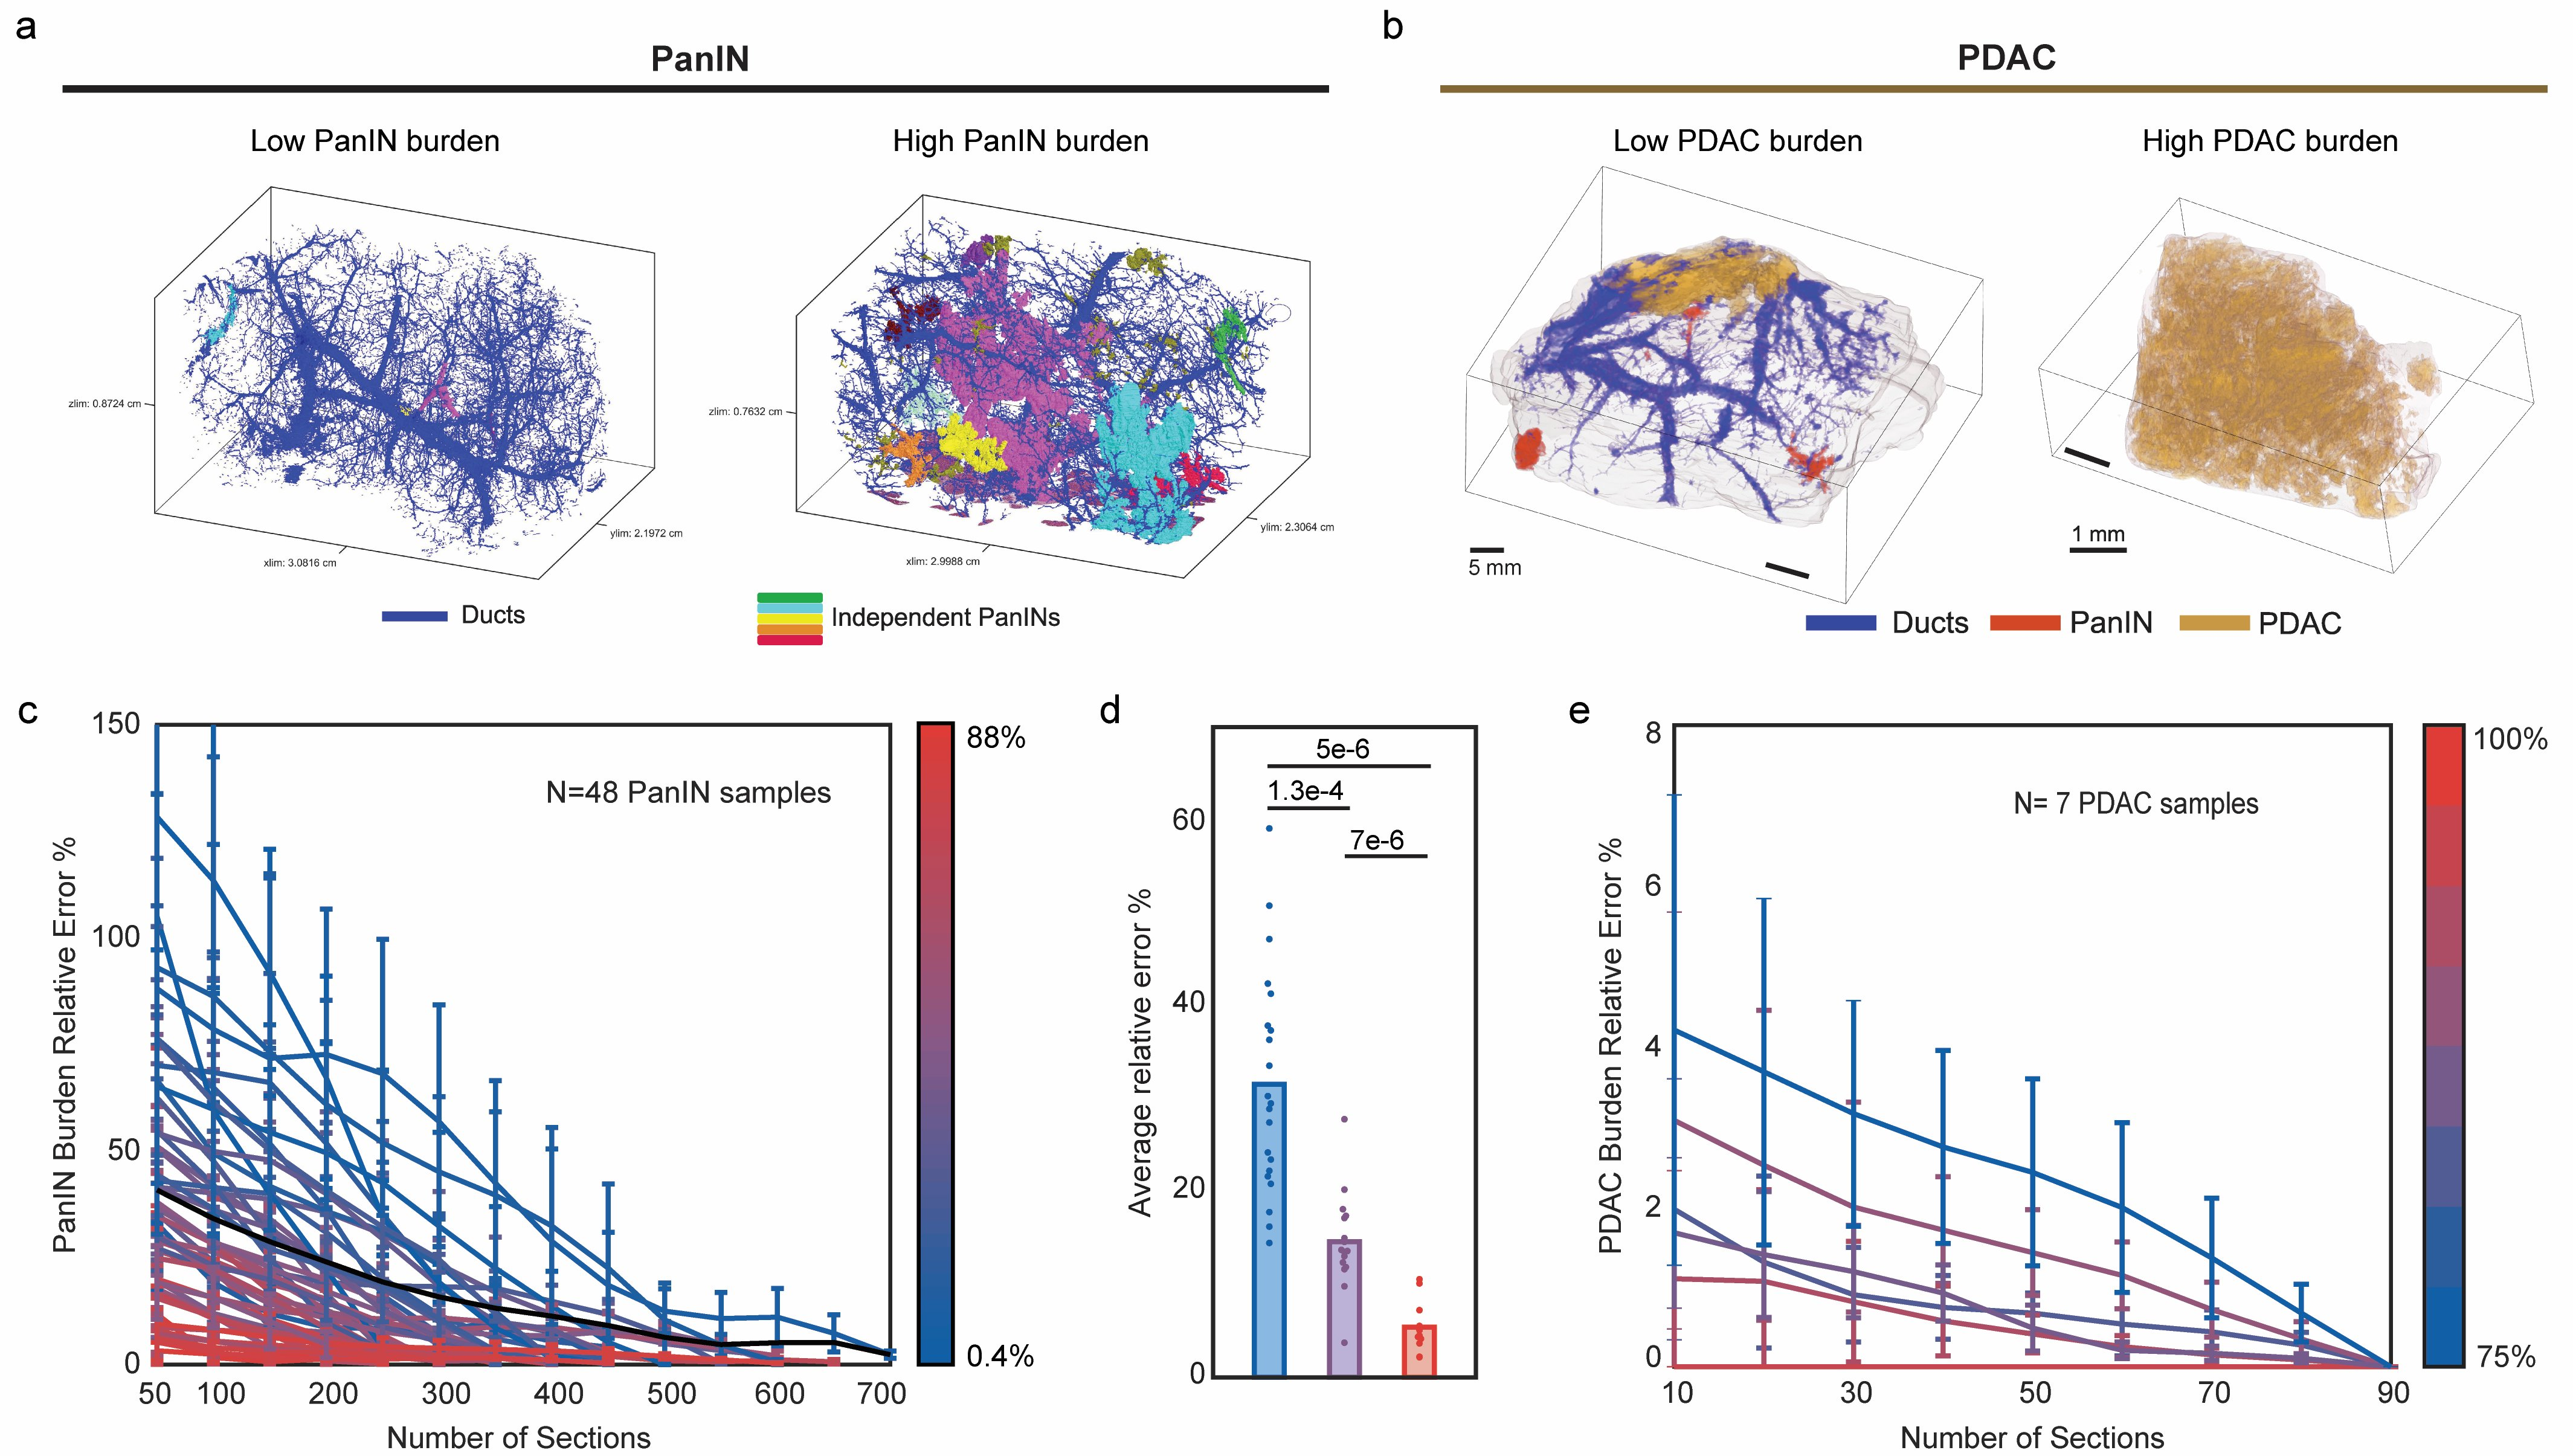
\includegraphics[width=\textwidth,clip,page=1] {figures/chapter2/PDAC_Fig_5.jpg}
            \caption{\textbf{Quantification of error in estimation of neoplastic content when subsampling 3D tissues.} 3D renderings of pancreata containing (a) low or high PanIN content and (b) low or high PDAC content. (c) For 48 3D samples containing PanINs (precursors to pancreatic cancer), the error in estimation of overall PanIN content plotted as a function of the number of consecutive sections subsampled. Lines color-coded according to the PanIN content of the 3D sample. (d) The data in (c) binned according to overall PanIN content to show that fewer sections are needed to accurately estimate the PanIN content of samples that contain many PanIN lesions, and vice versa. (e) The calculation of (c) repeated for the seven samples containing PDAC to show that fewer sections are needed to accurately estimate cancer content in samples that contain high cancer composition.}
            \label{chapter2_fig5}
        \end{center}
    \end{figure}

    
    
    \section{Discussion}
    Methods for spatially resolved cellular profiling have enabled in-depth quantitative mapping of tissues and tumors to study inter-patient and intra-patient differences in normal human anatomy and disease onset and progression. These methods profile extremely limited regions, which may impact the evaluation of tissue content and local heterogeneity due to tissue sub-sampling. 
    Here, we used CODA to quantitatively compare inter- and intra- sample heterogeneity through the lens of tissue composition. Using the pancreas as a model system, we demonstrated that correlation of tissue structures decays within tens of microns, even in normal tissues, that the target ROI selected by expert pathologists in design of tissue cores may be rapidly lost within tens of sections, and that tens of WSIs and hundreds of TMAs are needed to recapitulate the true, 3D tissue composition. Further, we demonstrated that quantification of 3D mapped tissues may be used to estimate the number of sections necessary for accurate 2D experimentation. Given that spatial heterogeneity is common in many tumors, similar patterns of rapid tissue structure decay and sampling challenges are also likely to be present in other cancers. To improve tissue analysis accuracy and reduce information loss, it is crucial to account for these subsampling factors.
    While this work studies inter- and intra- tumoral heterogeneity through meticulous enumeration of tissue composition, it is likely that molecular, genomic, and transcriptomic heterogeneity is also high within 3D tissue samples. For example, recent work has shown that PanIN (precursors to pancreatic cancer), exhibit great inter- and intra- lesional heterogeneity in KRAS mutations, suggesting that these lesions develop primarily from independent genetic events and may meet and merge within the ductal system.5,47 Using CyCIF to measure cellular heterogeneity, groups have also shown the alterations in marker-positive cells from TMAs to WSIs\cite{Lin2023Multiplexed}.
    The impact of transitioning from 2D to 3D analysis has been shown to be important in clinically relevant features, such as Gleason grade in prostate cancer, which can vary greatly across short distances of a 3D sample\cite{Liu2024Engineering,Koyuncu2023Visual,Bishop2024end,Lin2023Multiplexed,Song2024Analysis,Serafin2023Nondestructive,Marx2023Researchers,Coy20232D,Fukui2019Evaluation,Katsamenis2019X}. Additionally, recent work on pancreatic precursor lesions indicates that diagnostic criteria for intraductal papillary mucinous neoplasms (IPMN), primarily based on 2D planar cross-sectional dimensions, may be inaccurate when moving to 3D, potentially needing reclassification of some lesions as pancreatic intraepithelial neoplasias (PanINs)\cite{Kiemen2024PanIN}.
    Despite the potential of 3D imaging, its widespread adoption in basic and clinical research has been limited by high operational costs and the technical expertise necessary for sample processing, imaging, and computational analysis. However, several technological developments are reducing these barriers. The decreasing cost of chemical reagents for optical tissue clearing\cite{Lee2022MAX,Kim2022Optimized,Tomer2014Advanced,Glaser2019Multi,Ku2020Elasticizing}, optimized software\cite{Vladimirov2024Benchtop,Otomo2024descSPIM}, and the integration of generative artificial intelligence for interpolation of missing or damaged images in volumetric stacks are collectively enhancing scalability\cite{SaurabhInterpolAI}. In parallel, the emergence of open-source GUIs for light-sheet fluorescence microscopy and serial section histology reconstruction has accelerated the use of 3D in tissue analysis in biomedical and oncologic research\cite{Matos2025CODAvision,Marin2024navigate}.
    In sum, we demonstrate in this work that 3D assessments are necessary to accurately assess tissue composition and tumor content and provide guidelines for the rate of sampling necessary to rigorously assess spatially resolved tissue composition and associated tissue density and intercellular distances.
    
    \section{STAR Methods}

    \begin{table}[!h]
        \centering
        \renewcommand{\arraystretch}{1.3} % Add row spacing for readability
        \setlength{\tabcolsep}{6pt} % Adjust column spacing
        \captionsetup{justification=centering} % Centering the caption
        \caption{Star Methods Key Resource Table} % Add the legend text here
        \footnotesize % Reduce font size        
        \renewcommand{\arraystretch}{1.3} % Add row spacing
        \begin{tabularx}{\textwidth}{X X X} % Three equally wide columns
            \toprule
            \textbf{RESOURCE} & \textbf{SOURCE} & \textbf{IDENTIFIER} \\
            \midrule
            \multicolumn{3}{@{}l}{\textbf{Biological samples}} \\
            Tissue Microarray of human pancreas & TissueArray & PA803 \\
            Adult human pancreas & This paper & N/A \\
            \midrule
            \multicolumn{3}{@{}l}{\textbf{Chemicals, peptides, and recombinant proteins}} \\
            Molecular biology grade water & Corning & Catalog \#46-000-CI \\
            Xylene, Histological Grade & \href{https://www.sigmaaldrich.com}{Millipore Sigma} & Catalog \#534056 \\
            Hematoxylin Solution, Mayer’s & \href{https://www.sigmaaldrich.com}{Millipore Sigma} & Catalog \#MHS16 \\
            Bluing reagent & Dako & Catalog \#CS70230-2 \\
            Ethyl Alcohol, Pure (200 proof, anhydrous) & \href{https://www.sigmaaldrich.com}{Millipore Sigma} & Catalog \#E7023-500ML \\
            Eosin Y-solution, Alcoholic & \href{https://www.sigmaaldrich.com}{Millipore Sigma} & Catalog \#HT110116 \\
            \midrule
            \multicolumn{3}{@{}l}{\textbf{Deposited data}} \\
            3D human pancreas CODA blocks & This paper & \href{https://zenodo.org/records/15337577}{Zenodo: 15337577} \\
            \midrule
            \multicolumn{3}{@{}l}{\textbf{Software and algorithms}} \\
            OpenSlide & Goode et al. & \href{https://github.com/openslide/openslide}{GitHub: OpenSlide} \\
            ImageScope & Leica & \href{https://www.leicabiosystems.com/us/digital-pathology/manage/aperio-imagescope/}{Leica: ImageScope} \\
            CODA & Kiemen et al. & \href{https://zenodo.org/records/11130691}{Zenodo: 11130691} \\
            MATLAB & The MathWorks Inc. & \href{https://www.mathworks.com}{MathWorks website} \\
            \midrule
            \multicolumn{3}{@{}l}{\textbf{Other}} \\
            NanoZoomer S210 & Hamamatsu & Catalog \#C13239-01 \\
            \bottomrule
        \end{tabularx}
    \end{table}

    \section{Experimental model and study participant details}
    This retrospective study was approved by the Institutional Review Board (IRB) at the Johns Hopkins University School of Medicine. Human pancreatic tissue specimens were analyzed across three independent cohorts: a commercially acquired tissue microarray (TMA), whole-slide images (WSI), and a three-dimensionally reconstructed specimens processed using the CODA imaging pipeline\cite{Kiemen2022CODA}. All samples were obtained from archived, de-identified surgical resections and used in accordance with institutional ethical regulations and informed consent protocols.
    The TMA cohort consisted of 60 cores, each 1.5 mm in diameter, sampled from the pancreata of 30 individuals with pancreatic cancer. Each case was represented by two cores. The patients ranged in age from 40 to 84 years, with a mean of 58.4 years and a median of 60 years. Equal numbers of 30 male and 30 female donors were included in this group. These samples were obtained from a commercial vendor TissueArray. The WSI cohort comprises 64 surgical resections from patients treated at Johns Hopkins Hospital for pancreatic cancer, and is a cohort that was previously \cite{Fujikura2020Intraductal}. One representative FFPE slide per case was analyzed. Patient ages in this group ranged from 48 to 90 years, with a mean age of 64.4 years and a median age of 67 years. Of the patients, 22 were female and 25 were male, and gender information was not available for 17 individuals. The 3D-CODA cohort included pancreas resections from 14 individuals, also treated at Johns Hopkins Hospital, and is a cohort that was previously published\cite{Kiemen2022CODA,Hong2020Three}. Seven of these samples were processed using serial sectioning, computational alignment, and microanatomical segmentation for 3D reconstruction. The mean number of histological sections per case was 393 slides, with a total of 5,503 images across the cohort. Patient ages ranged from 41 to 75 years, with a mean of 61.4 and a median of 58 years. Six of the patients were female and eight were male. Histological. Sex and age data are summarized in Table S1. All tissue handling and data analysis procedures conformed to institutional and national research standards.
    
    \section{Method details}
    \subsection{Computational resources}
    For the execution of computational methods in this work, we used a computer with the following specifications: Intel i9 12th gen CPU, 128GB DDR4 memory RAM, and 3090 RTX Nvidia GPU. For implementation of the workflow by bench scientists, the CODA workflow has been modularly optimized to support scalability and accessibility, allowing streamlined execution on standard laptop configurations with reduced computational overhead\cite{Matos2025CODAvision}. 
    
    \subsection{Tissue processing}
    Resected tissues were formalin-fixed, paraffin embedded, and sectioned at a thickness of 4 µm. For the TMA and 2D-WSI cohorts, a single histological section was stained with H\&E. For the 3D-CODA cohort, a minimum of 270 serial sections were taken, and every third section was stained with H\&E, for a minimum of 90 H\&E-stained tissue sections per sample. H\&E-stained images were digitized at 20x magnification using a Hamamatsu S360 scanner.
    
    \subsection{Segmentation of pancreatic microanatomy in 2D}
    A previously developed deep learning semantic segmentation pipeline for the labelling of distinct microanatomical components in histological images was adapted here to label ten microanatomical components of human pancreatic cancer histology at 1 µm per pixel resolution: pancreatic cancer, pancreatic cancer precursor lesions, normal ductal epithelium, acinar tissue, islets of Langerhans, vasculature, nerves, fat, and extracellular matrix (ECM)\cite{Kiemen2022CODA,Chen2016DeepLab}. Convolutional neural networks were trained in MATLAB2023b to classify the TMA cores, 2D-WSI, and 3D-CODA cohorts of tissues. Manual annotations of the ten microanatomical tissue components were generated on a subset of histological images, and fed into the CODA-segmentation workflow for retraining of a resnet-50 network. Resulting networks were deemed acceptable if the overall accuracy exceeded 90\% and minimum per-class precision and recall exceeded 85\%.
    
    \subsection{Reconstruction of pancreatic microanatomy in 3D}
    CODA image registration was used to create digital tissue volumes from the serial H\&E images for the seven samples in the 3D-CODA cohort\cite{Kiemen2022CODA}. This nonlinear registration workflow iteratively aligns serial stacks of images (with the reference coordinates at the center of the stack), and utilizes a two-step global and local calculation in MATLAB2023b. Images are downsampled to a resolution of eight µm per pixel, converted to greyscale, and Gaussian-filtered. Global registration angle is calculated through maximization of the cross correlation of radon-transforms of the filtered images taken at discrete angles from 0 - 360°, and registration translation is calculated through maximization of the cross correlation of the rotated, filtered images. Local registration is computed by repeating this process along subsampled regions of the two globally registered images. This registration is repeated for all images in the serial samples and is subsequently rescaled and applied to the high resolution (1 µm per pixel resolution) H\&E and microanatomically segmented H\&E images.
    
    \subsection{Calculation of variation in tissue composition in 2D and 3D}
    For each discrete sample in the TMA, 2D-WSI and 3D-CODA cohort, overall microanatomical composition was assessed. First, the number of pixels classified as each of the 10 microanatomical tissue types segmented by the deep learning model was determined. Next, composition was defined as the area percent of each tissue type in each sample. Variation in tissue composition in the 2D-WSI cohort was defined as the distribution of composition of each tissue type segmented by the deep learning model. Variation in tissue composition in the 3D-CODA cohort was defined as the distribution of composition of each tissue type along the z-dimension of the serial stack of images, taking each serial histological image as an independent measurement. Minimum, maximum, mean, median, standard deviation, and histogram bin counts of each tissue component composition in the 2D-WSI and 3D-CODA cohorts were determined. In determination of the distribution of tissue composition in the 3D-CODA cohort, samples containing >90 serial images were randomly subsampled to contain 90 consecutive images.
    
    \subsection{Calculation of the number of tissue microarrays necessary to understand WSI and 3D tissue composition}
    Virtual TMAs (vTMAs) were generated in the 2D-WSI and 3D-CODA samples. First, a 2D or 3D coordinate was generated. Pixels were extracted corresponding to a 1 x 1 mm$^2$ square surrounding the coordinates. A circular filter was applied to this extracted square to leave a 1-mm diameter disk representing a vTMA taken from the 2D or 3D image. To determine the number of vTMAs necessary to accurately estimate the tissue composition of a WSI or 3D pancreatic cancer tissue sample, random coordinates were determined, virtual TMAs were generated, and the tissue composition of each vTMA was recorded. Error was calculated between the per-class vTMA tissue composition and the overall composition of the WSI or 3D tissue sample. Another random vTMA was generated, added to the first vTMA, and error was recalculated for the combined sampling of two vTMAs. This process was repeated for sampling of up to 800 vTMAs on the 3D tissue samples and up to 100 vTMAs on 2D-WSIs. One thousand such simulations were performed to determine the general trend of per-class TMA error in assessment of WSI and 3D sample tissue composition.
    
    \subsection{Calculation of the decay in spatial correlation within 2D and 3D samples}
    In each sample of the 3D-CODA cohort, 2D planes of pixels were extracted from each classified tissue volume. For each segmented tissue component, the cross-correlation of the pixels classified as that component in that plane to all other planes of the 3D-sample was determined, and this correlation along with the distance between the planes was recorded. This process was repeated for all possible combinations of z-planes in a volume, and was repeated for each of the seven tissue samples. Aggregate correlation of composition of a single tissue component as a function of distance within a 3D sample was defined as the mean cross-correlation of that tissue component across all images of all samples.
    
    \subsection{Calculation of the change in tissue composition along vTMA cores}
    Change in tissue composition along serial sections of a vTMA core was determined. First, manual selection of coordinates on the first image of a sample was selected corresponding to a region visibly seen to contain invasive cancer. Next, a virtual core was extracted from the 3D segmented tissue volume corresponding to a cylinder of 3 mm diameter. Serial vTMAs were taken from each core, and the tissue composition of each serial vTMA was determined. Error in composition of each tissue type between the initial, manually selected vTMA and each serial TMA was calculated, and recorded along with the section number of that virtual serial TMA. 
    
    \subsection{Calculation of the number of sections necessary to understand neoplastic content}
    Pancreatic neoplastic content was defined in two ways. For pancreatic cancer precursor lesions, PanIN content was defined as the volume of PanIN normalized by the combined volume of PanIN and normal ductal epithelium. For pancreatic cancer, PDAC content was defined as the volume of PDAC normalized by all PDAC, epithelial ducts, and PanIN total volume of the 3D sample. For each 3D sample, subvolumes were extracted corresponding to all combinations of between 1 and 90 serial tissue images. For each unique combination, the neoplastic content of the subvolume was calculated, and the relative error of this content was determined in relation to the neoplastic content of the whole 3D volume. For each 3D sample, measurements were grouped by the number of serial images contained in each subvolume.
    
    
    
    \subsection{Quantification and statistical analysis}
    All statistical analyses were performed using MATLAB scripts, with specific test employed as indicated. All significance tests were performed using the Wilcoxon rank sum test. To compare metrics within and between cohorts, median, mean, standard deviation, and interquartile range were determined. Relative error was defined as [measured value – expected value] / expected value. No other statistical calculations were performed in this work.
    
    \par
    \printbibliography[heading=subbibliography, title={References}]
\end{refsection}    
